% Options for packages loaded elsewhere
\PassOptionsToPackage{unicode}{hyperref}
\PassOptionsToPackage{hyphens}{url}
\documentclass[
  pandoc]{bxjsarticle}
\usepackage{xcolor}
\usepackage[margin=20mm]{geometry}
\usepackage{amsmath,amssymb}
\setcounter{secnumdepth}{5}
\usepackage{iftex}
\ifPDFTeX
  \usepackage[T1]{fontenc}
  \usepackage[utf8]{inputenc}
  \usepackage{textcomp} % provide euro and other symbols
\else % if luatex or xetex
  \usepackage{unicode-math} % this also loads fontspec
  \defaultfontfeatures{Scale=MatchLowercase}
  \defaultfontfeatures[\rmfamily]{Ligatures=TeX,Scale=1}
\fi
\usepackage{lmodern}
\ifPDFTeX\else
  % xetex/luatex font selection
\fi
% Use upquote if available, for straight quotes in verbatim environments
\IfFileExists{upquote.sty}{\usepackage{upquote}}{}
\IfFileExists{microtype.sty}{% use microtype if available
  \usepackage[]{microtype}
  \UseMicrotypeSet[protrusion]{basicmath} % disable protrusion for tt fonts
}{}
\makeatletter
\@ifundefined{KOMAClassName}{% if non-KOMA class
  \IfFileExists{parskip.sty}{%
    \usepackage{parskip}
  }{% else
    \setlength{\parindent}{0pt}
    \setlength{\parskip}{6pt plus 2pt minus 1pt}}
}{% if KOMA class
  \KOMAoptions{parskip=half}}
\makeatother
\setlength{\emergencystretch}{3em} % prevent overfull lines
\providecommand{\tightlist}{%
  \setlength{\itemsep}{0pt}\setlength{\parskip}{0pt}}
\usepackage{amsmath,amssymb}
\usepackage[most]{tcolorbox}
\usepackage{tikz}
\usetikzlibrary{arrows.meta, positioning}
\newcounter{question}
\newtcolorbox[use counter=question]{questionbox}[2][]{enhanced, breakable, colback=red!2!gray!3!white, colframe=red!50!gray, fonttitle=\bfseries, title={問\arabic{question}\ #2}, #1}
\newtcolorbox{answerbox}[2][]{enhanced, breakable, colback=green!2!gray!3!white, colframe=green!45!gray, fonttitle=\bfseries, title={問\ref{#2}の解答・解説}, #1}
\usepackage{titlesec}
\titleformat{\section}[display]{\normalfont\Large\bfseries}{【第\thesection 回】}{0.2em}{}
\titleformat{\subsection}[block]{\normalfont\large\bfseries}{\thesection-\arabic{subsection}.}{0.5em}{}
\newcommand{\ind}{\mathbf{1}}
\usepackage{bookmark}
\IfFileExists{xurl.sty}{\usepackage{xurl}}{} % add URL line breaks if available
\urlstyle{same}
\hypersetup{
  pdftitle={経営学への応用を目指すAI入門：数学演習問題集},
  pdfauthor={特殊講義1 補助資料},
  hidelinks,
  pdfcreator={LaTeX via pandoc}}

\title{経営学への応用を目指すAI入門：数学演習問題集}
\usepackage{etoolbox}
\makeatletter
\providecommand{\subtitle}[1]{% add subtitle to \maketitle
  \apptocmd{\@title}{\par {\large #1 \par}}{}{}
}
\makeatother
\subtitle{第1回〜第6回 講義内容完全準拠・論理展開追体験セット（完全版）}
\author{特殊講義1 補助資料}
\date{2026年5月17日（最終更新）}

\begin{document}
\maketitle

\begin{flushright}
\textbf{最終更新日：2026年5月17日 (v1.0)}
\end{flushright}

\section*{本演習問題集の進め方と活用法}\label{ux672cux6f14ux7fd2ux554fux984cux96c6ux306eux9032ux3081ux65b9ux3068ux6d3bux7528ux6cd5}
\addcontentsline{toc}{section}{本演習問題集の進め方と活用法}

本問題集は、講義スライドに登場する数式の「行間（省略された計算や証明）」を学生自身の手で動かして埋め、ブラックボックスを解消することを目的に設計されています。各セクションには講義スライドとの対応関係である\textbf{【該当内容】}と、その演習を行う目的である\textbf{【ねらい】}が記載されています。

また、各設問には以下の難易度が設定されています。

\begin{itemize}
\tightlist
\item
  \textbf{難易度：★0 (不要)} ：解き方が分かるなら解かなくてもいい。
\item
  \textbf{難易度：★1 (確認)}
  ：スライドの定義そのものの確認や、簡単な代入問題。
\item
  \textbf{難易度：★2 (基礎)}
  ：必須。講義の論理展開の行間を埋める標準的な問題。
\item
  \textbf{難易度：★3 (発展)} ：余裕があれば解くとよい。
\end{itemize}

\begin{center}\rule{0.5\linewidth}{0.5pt}\end{center}

\section{確率の基礎とリスク関数・ERM}\label{ux78baux7387ux306eux57faux790eux3068ux30eaux30b9ux30afux95a2ux6570erm}

\subsection{確率の基礎と期待値・分散の計算}\label{ux78baux7387ux306eux57faux790eux3068ux671fux5f85ux5024ux5206ux6563ux306eux8a08ux7b97}

\begin{questionbox}[label=q:1-indicator-function]{指示関数（Indicator function）の理解 \hfill \tcbox[enhanced, on line, boxsep=0pt, left=3pt, right=3pt, top=2pt, bottom=2pt, boxrule=0.5pt, arc=2pt, colback=white, opacityback=0, colframe=white, colupper=white, fontupper=\small\bfseries]{確認}\hspace{2pt}}

機械学習の理論（特に損失関数や分類問題の評価など）では、ある条件が満たされているか否かを表す\textbf{指示関数（定義関数）}
\(\ind\) が頻出する。条件（または事象） \(A\) に対して、指示関数
\(\ind\{A\}\) は以下のように定義される。 \[
\ind\{A\} = \begin{cases}
1 & (\text{条件 } A \text{ が真のとき}) \\
0 & (\text{条件 } A \text{ が偽のとき})
\end{cases}
\]

\begin{enumerate}
\def\labelenumi{\arabic{enumi}.}
\tightlist
\item
  \(x\) が次の値のとき、指示関数 \(\ind\{x \ge 1\}\)
  の値をそれぞれ求めよ。

  \begin{enumerate}
  \def\labelenumii{(\alph{enumii})}
  \tightlist
  \item
    \(x = 0\)
  \item
    \(x = 2\)
  \end{enumerate}
\item
  確率変数 \(Y := \ind\{X \ge 1\}\)
  の確率分布表（とり得る値と、それぞれの値をとる確率の表）の空欄（ア）〜（エ）を埋めよ。
\end{enumerate}

\begin{center}
\begin{tabular}{cc}
\(y\) & \(\mathbb{P}(Y=y)\) \\ \hline
（ア） & （ウ） \\
（イ） & （エ） \\
\end{tabular}
\end{center}

\hfill 

\hyperref[a:1-indicator-function]{（解答・解説へ）}

\end{questionbox}

\begin{questionbox}[label=q:1-discrete-expectation-variance]{離散型確率分布での期待値・分散計算 \hfill \tcbox[enhanced, on line, boxsep=0pt, left=3pt, right=3pt, top=2pt, bottom=2pt, boxrule=0.5pt, arc=2pt, colback=white, opacityback=0, colframe=white, colupper=white, fontupper=\small\bfseries]{不要}\hspace{2pt}}

ある離散確率変数 \(X\) は、確率 \(0.2\) で \(0\)、確率 \(0.5\) で
\(1\)、確率 \(0.3\) で \(2\) をとる。

\begin{enumerate}
\def\labelenumi{\arabic{enumi}.}
\tightlist
\item
  期待値 \(\mathbb{E}[X]\) を求めよ。
\item
  \(f(x) = x^2\) とするとき、期待値 \(\mathbb{E}[f(X)]\) を求めよ。
\item
  分散 \(\mathbb{V}[f(X)]\) を計算せよ。
\end{enumerate}

\hfill 

\hyperref[a:1-discrete-expectation-variance]{（解答・解説へ）}

\end{questionbox}

\begin{questionbox}[label=q:1-continuous-expectation-variance]{連続型確率分布での期待値・分散計算 \hfill \tcbox[enhanced, on line, boxsep=0pt, left=3pt, right=3pt, top=2pt, bottom=2pt, boxrule=0.5pt, arc=2pt, colback=white, opacityback=0, colframe=white, colupper=white, fontupper=\small\bfseries]{不要}\hspace{2pt}}

連続確率変数 \(X\) の確率密度関数 \(p(x)\) が、指示関数 \(\ind\)
を用いて実数全体 \(\mathbb{R}\) 上で以下のように定義されている。 \[
p(x) = 2x \cdot \ind\{0 \le x \le 1\}
\]

\begin{enumerate}
\def\labelenumi{\arabic{enumi}.}
\tightlist
\item
  \(\int_{-\infty}^\infty p(x) dx = 1\)
  （全確率が1）が満たされていることを示せ。
\item
  期待値 \(\mathbb{E}[X] = \int_{-\infty}^\infty x p(x) dx\)
  を計算せよ。
\item
  \(\mathbb{E}[X^2] = \int_{-\infty}^\infty x^2 p(x) dx\) を計算し、分散
  \(\mathbb{V}[X]\) を求めよ。
\end{enumerate}

\begin{center}\rule{0.5\linewidth}{0.5pt}\end{center}

\textbf{ヒント：}
\(\int_{-\infty}^\infty 2x \cdot \ind\{0 \le x \le 1\} dx = \int_0^1 2x dx\)
である。

\hfill 

\hyperref[a:1-continuous-expectation-variance]{（解答・解説へ）}

\end{questionbox}

\begin{tcolorbox}[enhanced, colback=blue!2!white, colframe=blue!60!black, fonttitle=\bfseries, drop shadow, title={【復習とヒント】期待値・分散・共分散の性質}]

\begin{itemize}
\tightlist
\item
  \textbf{線形性}:
  \(\mathbb{E}[aX + bY] = a\mathbb{E}[X] + b\mathbb{E}[Y]\)
\item
  \textbf{分散の定義}:
  \(\mathbb{V}[X] = \mathbb{E}[(X - \mathbb{E}[X])^2] = \mathbb{E}[X^2] - (\mathbb{E}[X])^2\)
\item
  \textbf{共分散の定義}:
  \(Cov(X,Y) = \mathbb{E}[(X - \mathbb{E}[X])(Y - \mathbb{E}[Y])]\)
\item
  \textbf{分散と共分散の関係}: \(\mathbb{V}[X] = Cov(X,X)\)
\item
  \textbf{共分散の双線形性}: \(Cov(aX+bY, Z) = aCov(X,Z) + bCov(Y,Z)\)
\end{itemize}

\end{tcolorbox}

\begin{questionbox}[label=q:1-variance-formula-proof]{共分散（Covariance）の2次形式的振る舞い \hfill \tcbox[enhanced, on line, boxsep=0pt, left=3pt, right=3pt, top=2pt, bottom=2pt, boxrule=0.5pt, arc=2pt, colback=white, opacityback=0, colframe=white, colupper=white, fontupper=\small\bfseries]{発展}\hspace{2pt}}

確率変数 \(X, Y, Z\) と定数 \(a, b\)
について、共分散の性質（双線形性・対称性） \begin{align*}
Cov(aX+bY, Z) &= a Cov(X,Z) + b Cov(Y,Z) \\
Cov(X,Y) &= Cov(Y,X)
\end{align*} を用いて、次の式を展開せよ。

\begin{enumerate}
\def\labelenumi{\arabic{enumi}.}
\tightlist
\item
  \(Cov(X, X+Y)\)
\item
  \(\mathbb{V}[aX + bY]\) （ヒント：\(\mathbb{V}[Z] = Cov(Z,Z)\)
  であることを利用せよ）
\end{enumerate}

\hfill 

\hyperref[a:1-variance-formula-proof]{（解答・解説へ）}

\end{questionbox}

\section{最適化と最小二乗法・偏微分}\label{ux6700ux9069ux5316ux3068ux6700ux5c0fux4e8cux4e57ux6cd5ux504fux5faeux5206}

\subsection{経験リスクの数式化（シグマを用いた書き下し）}\label{ux7d4cux9a13ux30eaux30b9ux30afux306eux6570ux5f0fux5316ux30b7ux30b0ux30deux3092ux7528ux3044ux305fux66f8ux304dux4e0bux3057}

\begin{questionbox}[label=q:2-empirical-risk-formulation]{経験リスクの立式 \hfill \tcbox[enhanced, on line, boxsep=0pt, left=3pt, right=3pt, top=2pt, bottom=2pt, boxrule=0.5pt, arc=2pt, colback=white, opacityback=0, colframe=white, colupper=white, fontupper=\small\bfseries]{必須}\hspace{2pt}}

\(n\) 個の訓練データ \(\{(x_i, y_i)\}_{i=1}^n\)
が与えられている。モデルクラスとして1次関数 \(f_{(w,b)}(x) = wx + b\)
を採用し、損失関数を二乗誤差 \(l(y, \hat{y}) = (y - \hat{y})^2\)
とするとき、経験リスク \(\hat{R}(f_{(w,b)})\) を書き下せ。

\hfill 

\hyperref[a:2-empirical-risk-formulation]{（解答・解説へ）}

\end{questionbox}

\begin{questionbox}[label=q:2-optimization-formulation-blank]{最適化問題の定式化：穴埋め \hfill \tcbox[enhanced, on line, boxsep=0pt, left=3pt, right=3pt, top=2pt, bottom=2pt, boxrule=0.5pt, arc=2pt, colback=white, opacityback=0, colframe=white, colupper=white, fontupper=\small\bfseries]{必須}\hspace{2pt}}

以下の最適化問題の定式化について、空欄 (ア) 〜 (エ)
に入る適切な数式や記号を答えよ。

\begin{enumerate}
\def\labelenumi{\arabic{enumi}.}
\tightlist
\item
  \textbf{【制約なし】} パラメータ \(\boldsymbol{\theta}\)
  を調整して、目的関数 \(L(\boldsymbol{\theta})\)
  を最小にする「最適なパラメータ
  \(\hat{\boldsymbol{\theta}}\)」を求める問題： \[
       \mathop{\mathrm{Min}}_{(ア)} (イ)
       \] ただし、\(\boldsymbol{\theta}\) が値をとる範囲は
  \(\mathbb{R}^d\) である。
\item
  \textbf{【制約あり】} パラメータの大きさ（L2ノルム）
  \(\|\boldsymbol{\theta}\|\) が定数 \(C\)
  を超えないという制約のもとで、目的関数 \(L(\boldsymbol{\theta})\)
  の最小値を求める問題： \[
       \mathop{\mathrm{Min}}_{(ウ)} (エ)
       \]
\end{enumerate}

\hfill 

\hyperref[a:2-optimization-formulation-blank]{（解答・解説へ）}

\end{questionbox}

\begin{questionbox}[label=q:2-erm-parameter-function]{目的関数のパラメータ関数化 \hfill \tcbox[enhanced, on line, boxsep=0pt, left=3pt, right=3pt, top=2pt, bottom=2pt, boxrule=0.5pt, arc=2pt, colback=white, opacityback=0, colframe=white, colupper=white, fontupper=\small\bfseries]{不要}\hspace{2pt}}

以下の2つのデータポイントが与えられている。

\begin{center}
\begin{tabular}{cc}
\(x\) & \(y\) \\ \hline
\(1\) & \(2\) \\
\(3\) & \(4\) \\
\end{tabular}
\end{center}

予測モデルを原点を通る直線 \(f_\theta(x) = \theta x\)
とし、損失関数を二乗誤差とする。このとき、経験リスク \[
\hat{R}(f_\theta) = \frac{1}{2} \sum_{i=1}^2 (y_i - f_\theta(x_i))^2
\] に具体的な数値を代入し、\(\theta\) の2次関数
\(A\theta^2 + B\theta + C\) の形に展開・整理せよ。

\hfill 

\hyperref[a:2-erm-parameter-function]{（解答・解説へ）}

\end{questionbox}

\subsection{最小二乗法の真髄：偏微分から一階の条件へ}\label{ux6700ux5c0fux4e8cux4e57ux6cd5ux306eux771fux9ac4ux504fux5faeux5206ux304bux3089ux4e00ux968eux306eux6761ux4ef6ux3078}

\begin{questionbox}[label=q:3-multivariate-gradient]{偏微分と勾配 \hfill \tcbox[enhanced, on line, boxsep=0pt, left=3pt, right=3pt, top=2pt, bottom=2pt, boxrule=0.5pt, arc=2pt, colback=white, opacityback=0, colframe=white, colupper=white, fontupper=\small\bfseries]{必須}\hspace{2pt}}

ベクトル \(\mathbf{w} = (w_1, w_2, w_3)^\top \in \mathbb{R}^3\)
に対する以下の関数 \(g(\mathbf{w})\) について、勾配
\(\nabla g(\mathbf{w})\) を求めよ。 \[
g(\mathbf{w}) = w_1^2 + 2w_2^2 + 3w_3^2 - 4w_1w_2 - 6w_2w_3
\]

\hfill 

\hyperref[a:3-multivariate-gradient]{（解答・解説へ）}

\end{questionbox}

\begin{questionbox}[label=q:2-partial-derivative-gradient]{線型単回帰モデルの最適パラメータ導出 \hfill \tcbox[enhanced, on line, boxsep=0pt, left=3pt, right=3pt, top=2pt, bottom=2pt, boxrule=0.5pt, arc=2pt, colback=white, opacityback=0, colframe=white, colupper=white, fontupper=\small\bfseries]{必須}\hspace{2pt}}

1次元の入力 \(x\) に対する線型単回帰モデル \(f_{w,b}(x) = wx + b\)
を考える。\(n\) 個の訓練データ \(\{(x_i, y_i)\}_{i=1}^n\)
に対する目的関数（経験リスク）を二乗誤差を用いて \[
L(w,b) = \frac{1}{n} \sum_{i=1}^n (y_i - (wx_i + b))^2
\] と定義する。この目的関数を最小化する最適なパラメータ
\((\hat{w}, \hat{b})\) を、以下の誘導に従って導出せよ。

\begin{enumerate}
\def\labelenumi{\arabic{enumi}.}
\tightlist
\item
  目的関数 \(L(w,b)\) を \(w\) および \(b\) について偏微分し、勾配
  \(\nabla L(w,b) = \begin{pmatrix} \frac{\partial L}{\partial w} \\ \frac{\partial L}{\partial b} \end{pmatrix}\)
  を求めよ。
\item
  一階の条件 \(\nabla L(w,b) = \mathbf{0}\) を用いて、パラメータ
  \(w, b\)
  に関する連立方程式を導き、それを行列とベクトルを用いた以下の形に整理せよ。
  \[
  \begin{pmatrix} ? & ? \\ ? & ? \end{pmatrix} \begin{pmatrix} w \\ b \end{pmatrix} = \begin{pmatrix} ? \\ ? \end{pmatrix}
  \]
\item
  上記の行列方程式を解くことで、最適なパラメータ \((\hat{w}, \hat{b})\)
  を求める式が \[
  \begin{pmatrix} \hat{w} \\ \hat{b} \end{pmatrix} = \begin{pmatrix} \sum_{i=1}^n x_i^2 & \sum_{i=1}^n x_i \\ \sum_{i=1}^n x_i & n \end{pmatrix}^{-1} \begin{pmatrix} \sum_{i=1}^n x_i y_i \\ \sum_{i=1}^n y_i \end{pmatrix}
  \] となることを示せ。
\end{enumerate}

\hfill 

\hyperref[a:2-partial-derivative-gradient]{（解答・解説へ）}

\end{questionbox}

\section{線型モデルの行列表現と正則化・モデル選択}\label{ux7ddaux578bux30e2ux30c7ux30ebux306eux884cux5217ux8868ux73feux3068ux6b63ux5247ux5316ux30e2ux30c7ux30ebux9078ux629e}

\subsection{ベクトルと行列の計算}\label{ux30d9ux30afux30c8ux30ebux3068ux884cux5217ux306eux8a08ux7b97}

\begin{questionbox}[label=q:3-matrix-vector-multiplication-practice]{行列・ベクトルの積の計算練習 \hfill \tcbox[enhanced, on line, boxsep=0pt, left=3pt, right=3pt, top=2pt, bottom=2pt, boxrule=0.5pt, arc=2pt, colback=white, opacityback=0, colframe=white, colupper=white, fontupper=\small\bfseries]{不要}\hspace{2pt}}

以下の行列・ベクトルの積を計算せよ。

\begin{enumerate}
\def\labelenumi{\arabic{enumi}.}
\tightlist
\item
  \textbf{【行列 \(\times\) 行列】} \[
  \begin{pmatrix} 1 & 2 \\ 3 & 4 \end{pmatrix} \begin{pmatrix} 2 & 0 & 1 \\ 1 & 3 & -1 \end{pmatrix}
  \]
\item
  \textbf{【行列 \(\times\) 縦ベクトル】} \[
  \begin{pmatrix} 1 & -1 & 2 \\ 0 & 3 & 1 \end{pmatrix} \begin{pmatrix} 2 \\ 1 \\ -1 \end{pmatrix}
  \]
\item
  \textbf{【横ベクトル \(\times\) 行列 \(\times\)
  縦ベクトル（二次形式）】} \[
  \begin{pmatrix} 1 & 2 \end{pmatrix} \begin{pmatrix} 2 & 0 \\ 0 & 3 \end{pmatrix} \begin{pmatrix} 1 \\ 2 \end{pmatrix}
  \]
\item
  \textbf{【横ベクトル \(\times\) 縦ベクトル（内積）】} \[
  \begin{pmatrix} 1 & 3 & -2 \end{pmatrix} \begin{pmatrix} 4 \\ -1 \\ 2 \end{pmatrix}
  \]
\item
  \textbf{【縦ベクトル \(\times\) 横ベクトル】} \[
  \begin{pmatrix} 2 \\ -1 \\ 3 \end{pmatrix} \begin{pmatrix} 1 & 4 \end{pmatrix}
  \]
\end{enumerate}

\hfill 

\hyperref[a:3-matrix-vector-multiplication-practice]{（解答・解説へ）}

\end{questionbox}

\begin{tcolorbox}[enhanced, colback=blue!2!white, colframe=blue!60!black, fonttitle=\bfseries, drop shadow, title={【復習とヒント】ベクトル・行列の掛け算の頻出パターン}]

ベクトルや行列の掛け算は、それぞれの「形状」を意識することで、結果がどのような形になるか（スカラー、ベクトル、行列）を視覚的に捉えることができます。

\begin{itemize}
\item
  \textbf{横ベクトル・縦ベクトルの掛け算 \(\rightarrow\)
  スカラーができる}

  \begin{center}
    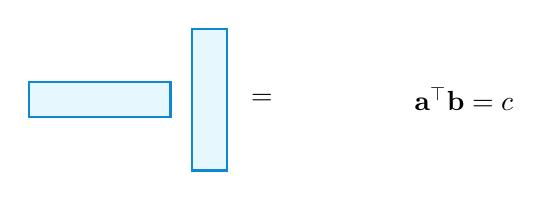
\begin{tikzpicture}[>=stealth, thick, scale=0.9, every node/.style={align=center}]
      \colorlet{vecbg}{cyan!10} \colorlet{vecborder}{cyan!70!blue}
      \draw[fill=vecbg, draw=vecborder] (0, -0.25) rectangle (2, 0.25) node[midway, font=\small] {ベクトル};
      \draw[fill=vecbg, draw=vecborder] (2.3, -1) rectangle (2.8, 1) node[midway, font=\small, align=center] {ベ\\ク\\ト\\ル};
      \node at (3.3, 0) {$=$};
      \node at (4.3, 0) {スカラー};
      \node[anchor=west] at (5.3, 0) {$\mathbf{a}^\top \mathbf{b} = c$};
    \end{tikzpicture}
    \end{center}
\item
  \textbf{縦ベクトル・横ベクトルの掛け算 \(\rightarrow\) 行列ができる}

  \begin{center}
    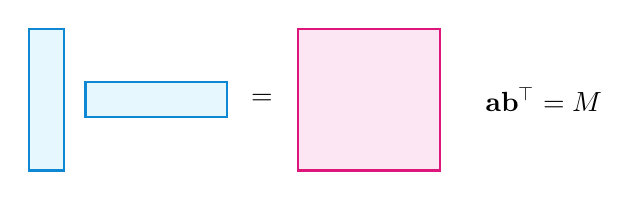
\begin{tikzpicture}[>=stealth, thick, scale=0.9, every node/.style={align=center}]
      \colorlet{vecbg}{cyan!10} \colorlet{vecborder}{cyan!70!blue}
      \colorlet{matbg}{magenta!10} \colorlet{matborder}{magenta!70!purple}
      \draw[fill=vecbg, draw=vecborder] (0, -1) rectangle (0.5, 1) node[midway, font=\small, align=center] {ベ\\ク\\ト\\ル};
      \draw[fill=vecbg, draw=vecborder] (0.8, -0.25) rectangle (2.8, 0.25) node[midway, font=\small] {ベクトル};
      \node at (3.3, 0) {$=$};
      \draw[fill=matbg, draw=matborder] (3.8, -1) rectangle (5.8, 1) node[midway, font=\small] {行列};
      \node[anchor=west] at (6.3, 0) {$\mathbf{a} \mathbf{b}^\top = M$};
    \end{tikzpicture}
    \end{center}
\item
  \textbf{行列を縦ベクトルに掛ける \(\rightarrow\) 縦ベクトルになる}

  \begin{center}
    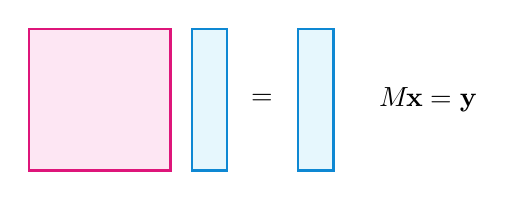
\begin{tikzpicture}[>=stealth, thick, scale=0.9, every node/.style={align=center}]
      \colorlet{vecbg}{cyan!10} \colorlet{vecborder}{cyan!70!blue}
      \colorlet{matbg}{magenta!10} \colorlet{matborder}{magenta!70!purple}
      \draw[fill=matbg, draw=matborder] (0, -1) rectangle (2, 1) node[midway, font=\small] {行列};
      \draw[fill=vecbg, draw=vecborder] (2.3, -1) rectangle (2.8, 1) node[midway, font=\small, align=center] {ベ\\ク\\ト\\ル};
      \node at (3.3, 0) {$=$};
      \draw[fill=vecbg, draw=vecborder] (3.8, -1) rectangle (4.3, 1) node[midway, font=\small, align=center] {ベ\\ク\\ト\\ル};
      \node[anchor=west] at (4.8, 0) {$M \mathbf{x} = \mathbf{y}$};
    \end{tikzpicture}
    \end{center}
\item
  \textbf{横ベクトル・行列・縦ベクトルの順に掛ける \(\rightarrow\)
  スカラーになる}

  \begin{center}
    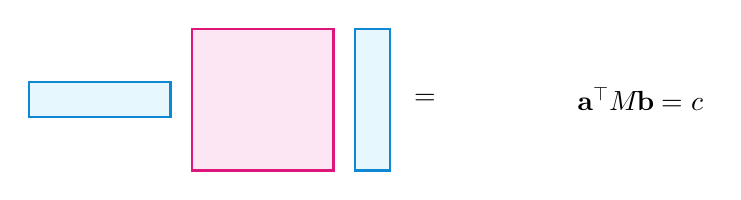
\begin{tikzpicture}[>=stealth, thick, scale=0.9, every node/.style={align=center}]
      \colorlet{vecbg}{cyan!10} \colorlet{vecborder}{cyan!70!blue}
      \colorlet{matbg}{magenta!10} \colorlet{matborder}{magenta!70!purple}
      \draw[fill=vecbg, draw=vecborder] (0, -0.25) rectangle (2, 0.25) node[midway, font=\small] {ベクトル};
      \draw[fill=matbg, draw=matborder] (2.3, -1) rectangle (4.3, 1) node[midway, font=\small] {行列};
      \draw[fill=vecbg, draw=vecborder] (4.6, -1) rectangle (5.1, 1) node[midway, font=\small, align=center] {ベ\\ク\\ト\\ル};
      \node at (5.6, 0) {$=$};
      \node at (6.6, 0) {スカラー};
      \node[anchor=west] at (7.6, 0) {$\mathbf{a}^\top M \mathbf{b} = c$};
    \end{tikzpicture}
    \end{center}
\end{itemize}

【注意】いずれも、行列やベクトルの形状が掛け算可能なように整合していることを前提としています。

\end{tcolorbox}

\begin{questionbox}[label=q:3-matrix-vector-patterns]{ベクトル・行列の積の頻出パターンと成分表示 \hfill \tcbox[enhanced, on line, boxsep=0pt, left=3pt, right=3pt, top=2pt, bottom=2pt, boxrule=0.5pt, arc=2pt, colback=white, opacityback=0, colframe=white, colupper=white, fontupper=\small\bfseries]{必須}\hspace{2pt}}

講義スライドで登場した行列・ベクトルの積に関する視覚的なパターンの意味を、成分表示を用いて確認せよ。

\begin{enumerate}
\def\labelenumi{\arabic{enumi}.}
\item
  \textbf{【横ベクトル \(\times\) 縦ベクトル \(\to\) 内積】} \[
  \mathbf{a}^\top \mathbf{b} =
  \begin{pmatrix} a_1 & a_2 & \dots & a_d \end{pmatrix}
  \begin{pmatrix} b_1 \\ b_2 \\ \vdots \\ b_d \end{pmatrix}
  = c
  \] この結果 \(c\) が内積
  \(\langle \mathbf{a}, \mathbf{b} \rangle = a_1b_1 + \dots + a_db_d\)
  と一致することを、成分計算により確認せよ。また、同様にして
  \(\mathbf{a}^\top \mathbf{b} = \mathbf{b}^\top \mathbf{a}\)
  となること（内積の順序の入れ替え可能性）も確認せよ。ただし、\(1\times 1\)行列はスカラーと同一視してよい。
\item
  \textbf{【行列 \(\times\) 縦ベクトル \(\to\) 縦ベクトル】} 行列
  \(B \in \mathbb{R}^{m \times d}\)
  を、横ベクトルを縦に並べたブロック行列、および縦ベクトルを横に並べたブロック行列としてそれぞれ解釈する。つまり、
  \[
  B = \begin{pmatrix} B_{11} & \dots & B_{1d} \\ \vdots & \ddots & \vdots \\ B_{m1} & \dots & B_{md} \end{pmatrix}
  = \begin{pmatrix} \quad \mathbf{b}_1^\top \quad \\ \vdots \\ \quad \mathbf{b}_m^\top \quad \end{pmatrix}
  = \begin{pmatrix} \boldsymbol{\beta}_1 & \cdots & \boldsymbol{\beta}_d \end{pmatrix}
  \] と捉えるとき、縦ベクトル \(\mathbf{v} \in \mathbb{R}^d\) との積
  \(B\mathbf{v}\)
  について次の等式がそれぞれ成り立つことを成分計算により確認せよ。

  \begin{itemize}
  \item
    \textbf{横ベクトルが縦に並んでいるとみなす場合（内積の縦並び）：} \[
    B\mathbf{v} =
    \begin{pmatrix} \quad \mathbf{b}_1^\top \quad \\ \vdots \\ \quad \mathbf{b}_m^\top \quad \end{pmatrix} \mathbf{v}
    = \begin{pmatrix} \mathbf{b}_1^\top \mathbf{v} \\ \vdots \\ \mathbf{b}_m^\top \mathbf{v} \end{pmatrix}
    \]
  \item
    \textbf{縦ベクトルが横に並んでいるとみなす場合（列ベクトルの重み付き和）：}
    \[
    B\mathbf{v} =
    \begin{pmatrix} \boldsymbol{\beta}_1 & \cdots & \boldsymbol{\beta}_d \end{pmatrix}
    \begin{pmatrix} v_1 \\ \vdots \\ v_d \end{pmatrix}
    = v_1 \boldsymbol{\beta}_1 + \cdots + v_d \boldsymbol{\beta}_d
    \]
  \end{itemize}
\end{enumerate}

\hfill 

\hyperref[a:3-matrix-vector-patterns]{（解答・解説へ）}

\end{questionbox}

\begin{tcolorbox}[enhanced, colback=blue!2!white, colframe=blue!60!black, fonttitle=\bfseries, drop shadow, title={【復習とヒント】ベクトル・行列の積のコツ}]

行列は、いくつかの計算パターンでは、行（横ベクトル）や列（縦ベクトル）が並んだものとしてイメージすると、複雑な計算も直感的に捉えやすくなります。

\begin{itemize}
\item
  \textbf{行列の行ベクトル・列ベクトル表現}
  行列は横ベクトルが縦に並んだものとも、縦ベクトルが横に並んだものとも思えます。

  \begin{center}
    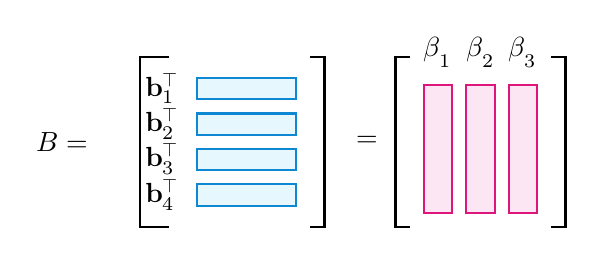
\begin{tikzpicture}[>=stealth, thick, scale=0.9, every node/.style={align=center}]
      \colorlet{vecbg}{cyan!10} \colorlet{vecborder}{cyan!70!blue}
      \colorlet{colbg}{magenta!10} \colorlet{colborder}{magenta!70!purple}

      \node at (-1.5, 0) {$B =$};
      \draw[draw=black, thick] (0, 1.2) -- (-0.4, 1.2) -- (-0.4, -1.2) -- (0, -1.2);
      \draw[draw=black, thick] (2.0, 1.2) -- (2.2, 1.2) -- (2.2, -1.2) -- (2.0, -1.2);
      \foreach \y/\i in {0.75/1, 0.25/2, -0.25/3, -0.75/4} {
        \node[anchor=east] at (0.3, \y) {$\mathbf{b}_\i^\top$};
        \draw[fill=vecbg, draw=vecborder] (0.4, \y-0.15) rectangle (1.8, \y+0.15);
      }
      \node at (2.8, 0) {$=$};
      \draw[draw=black, thick] (3.4, 1.2) -- (3.2, 1.2) -- (3.2, -1.2) -- (3.4, -1.2);
      \draw[draw=black, thick] (5.4, 1.2) -- (5.6, 1.2) -- (5.6, -1.2) -- (5.4, -1.2);
      \foreach \x/\i in {3.8/1, 4.4/2, 5.0/3} {
        \node[anchor=south] at (\x, 0.9) {$\boldsymbol{\beta}_\i$};
        \draw[fill=colbg, draw=colborder] (\x-0.2, -1.0) rectangle (\x+0.2, 0.8);
      }
    \end{tikzpicture}
    \end{center}
\item
  \textbf{横ベクトルが縦に並んでいると思うと}
  各「横成分」に右のベクトルが分配されたように振る舞います。

  \begin{center}
    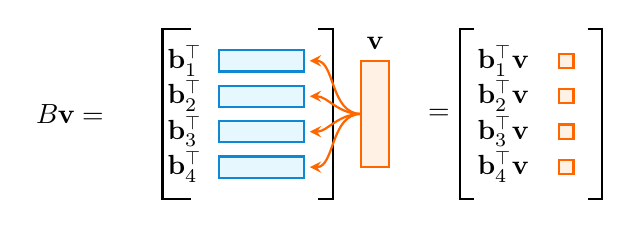
\begin{tikzpicture}[>=stealth, thick, scale=0.9, every node/.style={align=center}]
      \colorlet{vecbg}{cyan!10} \colorlet{vecborder}{cyan!70!blue}
      \colorlet{vbg}{orange!10} \colorlet{vborder}{orange!80!red}

      \node at (-1.7, 0) {$B \mathbf{v} =$};
      \draw[draw=black, thick] (0, 1.2) -- (-0.4, 1.2) -- (-0.4, -1.2) -- (0, -1.2);
      \draw[draw=black, thick] (1.8, 1.2) -- (2.0, 1.2) -- (2.0, -1.2) -- (1.8, -1.2);
      \foreach \y/\i in {0.75/1, 0.25/2, -0.25/3, -0.75/4} {
        \node[anchor=east] at (0.3, \y) {$\mathbf{b}_\i^\top$};
        \draw[fill=vecbg, draw=vecborder] (0.4, \y-0.15) rectangle (1.6, \y+0.15);
      }
      \draw[fill=vbg, draw=vborder] (2.4, -0.75) rectangle (2.8, 0.75);
      \node at (2.6, 1.0) {$\mathbf{v}$};
      \foreach \y in {0.75, 0.25, -0.25, -0.75} {
        \draw[->, orange!80!red, shorten >=2pt] (2.4, 0) to[out=180, in=0] (1.6, \y);
      }
      \node at (3.5, 0) {$=$};
      \draw[draw=black, thick] (4.0, 1.2) -- (3.8, 1.2) -- (3.8, -1.2) -- (4.0, -1.2);
      \draw[draw=black, thick] (5.6, 1.2) -- (5.8, 1.2) -- (5.8, -1.2) -- (5.6, -1.2);
      \foreach \y/\i in {0.75/1, 0.25/2, -0.25/3, -0.75/4} {
        \node[anchor=west] at (3.9, \y) {$\mathbf{b}_\i^\top \mathbf{v}$};
        \draw[fill=vbg, draw=vborder] (5.2, \y-0.1) rectangle (5.4, \y+0.1);
      }
    \end{tikzpicture}
    \end{center}
\item
  \textbf{縦ベクトルが横に並んでいると思うと}
  あたかも通常のベクトル間の内積（成分同士を掛けて足す）かのように振る舞います。

  \begin{center}
    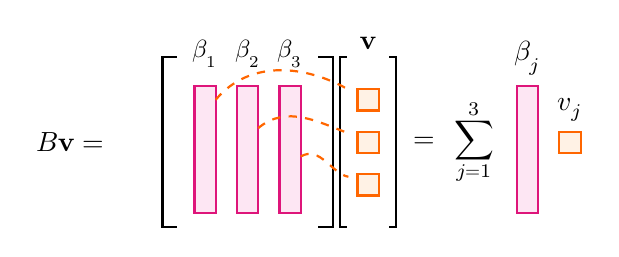
\begin{tikzpicture}[>=stealth, thick, scale=0.9, every node/.style={align=center}]
      \colorlet{colbg}{magenta!10} \colorlet{colborder}{magenta!70!purple}
      \colorlet{vbg}{orange!10} \colorlet{vborder}{orange!80!red}

      \node at (-1.5, 0) {$B \mathbf{v} =$};
      \draw[draw=black, thick] (0, 1.2) -- (-0.2, 1.2) -- (-0.2, -1.2) -- (0, -1.2);
      \draw[draw=black, thick] (2.0, 1.2) -- (2.2, 1.2) -- (2.2, -1.2) -- (2.0, -1.2);
      \foreach \x/\i in {0.4/1, 1.0/2, 1.6/3} {
        \node[anchor=south, inner sep=1pt] at (\x, 1.0) {\small $\boldsymbol{\beta}_\i$};
        \draw[fill=colbg, draw=colborder] (\x-0.15, -1.0) rectangle (\x+0.15, 0.8);
      }
      \draw[draw=black, thick] (2.4, 1.2) -- (2.3, 1.2) -- (2.3, -1.2) -- (2.4, -1.2);
      \draw[draw=black, thick] (3.0, 1.2) -- (3.1, 1.2) -- (3.1, -1.2) -- (3.0, -1.2);
      \node at (2.7, 1.4) {$\mathbf{v}$};
      \foreach \y/\i in {0.6/1, 0.0/2, -0.6/3} {
        \draw[fill=vbg, draw=vborder] (2.55, \y-0.15) rectangle (2.85, \y+0.15);
      }
      \draw[dashed, orange!80!red, shorten >=2pt, thick] (0.55, 0.6) to[out=50, in=150] (2.5, 0.7);
      \draw[dashed, orange!80!red, shorten >=2pt, thick] (1.15, 0.2) to[out=40, in=160] (2.5, 0.1);
      \draw[dashed, orange!80!red, shorten >=2pt, thick] (1.75, -0.2) to[out=30, in=170] (2.5, -0.5);

      \node at (3.5, 0) {$=$};
      \node at (4.2, 0) {$\displaystyle \sum_{j=1}^3$};
      \draw[fill=colbg, draw=colborder] (4.8, -1.0) rectangle (5.1, 0.8);
      \node[anchor=south] at (4.95, 0.8) {$\boldsymbol{\beta}_j$};
      \draw[fill=vbg, draw=vborder] (5.4, -0.15) rectangle (5.7, 0.15);
      \node[anchor=south] at (5.55, 0.15) {$v_j$};
    \end{tikzpicture}
    \end{center}
\end{itemize}

\end{tcolorbox}

\subsection{ベクトルの内積と性質}\label{ux30d9ux30afux30c8ux30ebux306eux5185ux7a4dux3068ux6027ux8cea}

\begin{tcolorbox}[enhanced, colback=blue!2!white, colframe=blue!60!black, fonttitle=\bfseries, drop shadow, title={【復習とヒント】ベクトルの内積の主な出番}]

内積の主な出番は3つあります。 内積は \(\langle \cdot, \cdot \rangle\) や
\(\mathbf{x}^\top \mathbf{y}\) で表します。

\begin{itemize}
\item
  \textbf{重み付き和を簡潔に表す}（成分ごとの重み
  \(\mathbf{w} = (w_1, \dots, w_d)^\top\)）
  \[ \mathbf{w}^\top \mathbf{x} = w_1 x_1 + \dots + w_d x_d \]
\item
  \textbf{2つのベクトルの向きの揃い具合}（同じ向きで最大、逆向きで最小）
  長さ1のベクトル同士なら、
  \[ \langle \textcolor{orange!80!red}{\nwarrow}, \textcolor{green!70!black}{\searrow} \rangle = -1, \quad \langle \textcolor{orange!80!red}{\nwarrow}, \textcolor{green!70!black}{\nearrow} \rangle = 0, \quad \langle \textcolor{orange!80!red}{\nwarrow}, \textcolor{green!70!black}{\nwarrow} \rangle = 1 \quad \text{（長さ1の場合）} \]
  【補足】同じ向きを向いている場合に内積が最も大きくなるという主張はコーシー・シュワルツの不等式から従う。ここでベクトルの長さは
  \(\|\cdot\| = \sqrt{\langle\cdot, \cdot\rangle}\) で測る。
\item
  \textbf{特定の方向の成分の抽出}（ベクトル \(\mathbf{a}\) の「ベクトル
  \(\mathbf{b}\) 方向成分」）
  \[ \mathbf{a} = \frac{\langle \mathbf{a}, \mathbf{b} \rangle}{\langle \mathbf{b}, \mathbf{b} \rangle} \mathbf{b} + (\mathbf{b}\text{に直交する成分}) \]

  \begin{center}
    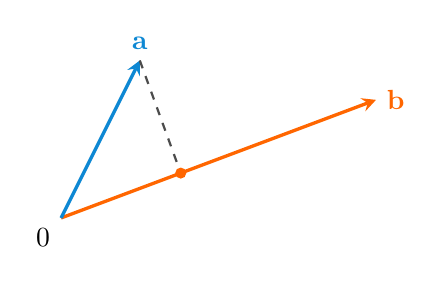
\begin{tikzpicture}[>=stealth, thick, scale=1.0]
      \draw[->, orange!80!red, line width=1.2pt] (0,0) -- (4,1.5) node[right] {$\mathbf{b}$};
      \draw[->, cyan!70!blue, line width=1.2pt] (0,0) -- (1,2) node[above] {$\mathbf{a}$};
      \draw[dashed, black!70] (1,2) -- (1.52,0.57);
      \fill[orange!80!red] (1.52,0.57) circle (2pt);
      \node[below left] at (0,0) {$0$};
    \end{tikzpicture}
    \end{center}

  【補足】最後の
  \(\mathbf{a} = \frac{\langle \mathbf{a}, \mathbf{b} \rangle}{\langle \mathbf{b}, \mathbf{b} \rangle} \mathbf{b} + (\mathbf{b}\text{に直交する成分})\)
  という分解は、\(\langle \mathbf{a} - \frac{\langle \mathbf{a}, \mathbf{b} \rangle}{\langle \mathbf{b}, \mathbf{b} \rangle} \mathbf{b}, \mathbf{b} \rangle = 0\)
  により確かめられる。
\end{itemize}

\end{tcolorbox}

\begin{questionbox}[label=q:3-inner-product-roles]{内積の役割と計算 \hfill \tcbox[enhanced, on line, boxsep=0pt, left=3pt, right=3pt, top=2pt, bottom=2pt, boxrule=0.5pt, arc=2pt, colback=white, opacityback=0, colframe=white, colupper=white, fontupper=\small\bfseries]{不要}\hspace{2pt}}

以下の小問に答えよ。

\begin{enumerate}
\def\labelenumi{\arabic{enumi}.}
\tightlist
\item
  \textbf{【重み付き和の計算】} ある商品の3つの特徴量が
  \(\mathbf{x} = (2, -1, 4)^\top\) であり、各特徴量に対する重みが
  \(\mathbf{w} = (3, 2, 1)^\top\) であるとする。この商品のスコアを内積
  \(\mathbf{w}^\top \mathbf{x}\) として計算せよ。
\item
  \textbf{【ベクトルの揃い具合と直交性 (1)】} 長さが1のベクトル
  \(\mathbf{a} = (\frac{2}{3}, \frac{2}{3}, \frac{1}{3})^\top\) と
  \(\mathbf{b} = (\frac{2}{3}, -\frac{1}{3}, -\frac{2}{3})^\top\)
  について、内積 \(\mathbf{a}^\top \mathbf{b}\)
  を計算し、これら2つのベクトルの幾何学的な位置関係（同じ方向、真逆の方向、直交、それらのどれでもない、のいずれか）を特定せよ。
\item
  \textbf{【ベクトルの揃い具合と直交性 (2)】} 長さが1のベクトル
  \(\mathbf{a} = (\frac{2}{3}, \frac{2}{3}, \frac{1}{3})^\top\) と
  \(\mathbf{c} = (\frac{1}{3}, \frac{2}{3}, \frac{2}{3})^\top\)
  について、内積 \(\mathbf{a}^\top \mathbf{c}\)
  を計算し、位置関係（同じ方向、真逆の方向、直交、それらのどれでもない、のいずれか）を特定せよ。
\item
  \textbf{【直交分解の係数】} ベクトル \(\mathbf{x} = (5, 2, -1)^\top\)
  と \(\mathbf{u} = (1, -1, 2)^\top\) がある。ベクトル \(\mathbf{x}\)
  を、\(\mathbf{u}\) と平行な成分と \(\mathbf{u}\) に直交する成分
  \(\mathbf{v}\) を用いて
  \[ \mathbf{x} = \beta \mathbf{u} + \mathbf{v} \quad (\mathbf{v} \text{ は } \mathbf{u} \text{ と直交}) \]
  と分解するとき、係数 \(\beta\) を内積を用いて求めよ。
\end{enumerate}

\hfill 

\hyperref[a:3-inner-product-roles]{（解答・解説へ）}

\end{questionbox}

\subsection{パラメータ線型モデルの表現（特徴写像）}\label{ux30d1ux30e9ux30e1ux30fcux30bfux7ddaux578bux30e2ux30c7ux30ebux306eux8868ux73feux7279ux5fb4ux5199ux50cf}

\begin{questionbox}[label=q:3-polynomial-feature-mapping]{多項式特徴写像による線型表現 \hfill \tcbox[enhanced, on line, boxsep=0pt, left=3pt, right=3pt, top=2pt, bottom=2pt, boxrule=0.5pt, arc=2pt, colback=white, opacityback=0, colframe=white, colupper=white, fontupper=\small\bfseries]{確認}\hspace{2pt}}

1次元の入力 \(x\) に対し、特徴写像を
\(\boldsymbol{\phi}(x) = (1, x, x^2)^\top\) と定義する。
パラメータベクトルを
\(\boldsymbol{\theta} = (\theta_0, \theta_1, \theta_2)^\top\) とする。

\begin{enumerate}
\def\labelenumi{\arabic{enumi}.}
\tightlist
\item
  線型モデル \(f(x) = \boldsymbol{\theta}^\top \boldsymbol{\phi}(x)\)
  を書き下せ。
\item
  このモデルは、パラメータ \(\boldsymbol{\theta}\)
  に着目すると何次式か。また、入力 \(x\) に着目すると何次式か答えよ。
  （ただし，多変数多項式の次数は，最大の単項式の次数のことである．）
\end{enumerate}

\hfill 

\hyperref[a:3-polynomial-feature-mapping]{（解答・解説へ）}

\end{questionbox}

\begin{questionbox}[label=q:3-bag-of-words-representation]{テキストデータへの適用（Bag-of-Words）と最小二乗法 \hfill \tcbox[enhanced, on line, boxsep=0pt, left=3pt, right=3pt, top=2pt, bottom=2pt, boxrule=0.5pt, arc=2pt, colback=white, opacityback=0, colframe=white, colupper=white, fontupper=\small\bfseries]{必須}\hspace{2pt}}

テキストの文書分類や数値予測を行う際、文書中の単語の出現頻度をもとに特徴ベクトルを作る手法を\textbf{Bag-of-Words}と呼びます。

今、以下の4つのテキスト（文書）と、それぞれの正解ラベル（重要度スコアなど）の表が与えられているとします。

\smallskip
\begin{center}
\begin{tabular}{|c|p{9cm}|c|}
\hline
文書番号 ($i$) & \multicolumn{1}{c|}{文書の内容 ($x_i$)} & 正解ラベル ($y_i$) \\
\hline
1 & 最新の AI 技術は急速に発展しています。多くの研究者が新しい AI モデルを開発しています。 & 5 \\
2 & 今朝の人気ニュース番組で、有名な俳優の最新映画が紹介されました。多くのファンが劇場に詰めかけています。 & 0 \\
3 & AI の活用はビジネスに変革をもたらします。企業経営において AI を導入するビジネス戦略が不可欠です。 & 10 \\
4 & ペット関連のビジネスが盛んです。特に犬向けのサービスは市場規模が拡大しています。 & 15 \\
\hline
\end{tabular}
\end{center}
\smallskip

特徴ベクトル \(\boldsymbol{\phi}(x)\) を以下のように定義します。 \[
\boldsymbol{\phi}(x) = \begin{pmatrix} \text{「AI」の出現回数} \\ \text{「ビジネス」の出現回数} \\ \text{「犬」の出現回数} \end{pmatrix}
\]

この特徴ベクトルを用いた線型モデル
\(f(x) = \boldsymbol{\theta}^\top \boldsymbol{\phi}(x)\) （ただし
\(\boldsymbol{\theta} = (\theta_1, \theta_2, \theta_3)^\top\)）について、以下の問いに答えよ。

\begin{enumerate}
\def\labelenumi{\arabic{enumi}.}
\tightlist
\item
  各文書 \(x_1, x_2, x_3, x_4\) に対応する特徴ベクトル
  \(\boldsymbol{\phi}(x_1), \boldsymbol{\phi}(x_2), \boldsymbol{\phi}(x_3), \boldsymbol{\phi}(x_4)\)
  をそれぞれ具体的に求めよ。
\item
  計画行列 \(\Phi \in \mathbb{R}^{4 \times 3}\) と、ラベルベクトル
  \(\mathbf{y} \in \mathbb{R}^4\) をそれぞれ具体的に数値で書き下せ。
  なお，計画行列とは，ここでは，
  \[\Phi = \begin{pmatrix} \boldsymbol{\phi}(x_1)^\top \\ \boldsymbol{\phi}(x_2)^\top \\ \boldsymbol{\phi}(x_3)^\top \\ \boldsymbol{\phi}(x_4)^\top \end{pmatrix}\]
  のことである．
\item
  このモデルに対して、最小二乗誤差の意味で最適なパラメータ
  \(\hat{\boldsymbol{\theta}}\) を求める一般式を、計画行列 \(\Phi\)
  とラベルベクトル \(\mathbf{y}\)
  を用いて（逆行列の記号を用いて）書き下せ。 （ただし，この設定において
  \(\Phi^\top \Phi\) の逆行列が存在することは認めてよい．）
\end{enumerate}

\hfill 

\hyperref[a:3-bag-of-words-representation]{（解答・解説へ）}

\end{questionbox}

\subsection{多変数関数の経験リスクと勾配}\label{ux591aux5909ux6570ux95a2ux6570ux306eux7d4cux9a13ux30eaux30b9ux30afux3068ux52feux914d}

\begin{questionbox}[label=q:3-multivariate-empirical-risk]{3変数パラメータの経験リスク \hfill \tcbox[enhanced, on line, boxsep=0pt, left=3pt, right=3pt, top=2pt, bottom=2pt, boxrule=0.5pt, arc=2pt, colback=white, opacityback=0, colframe=white, colupper=white, fontupper=\small\bfseries]{確認}\hspace{2pt}}

3つのデータポイント \((x_1, y_1) = (1, 2)\), \((x_2, y_2) = (2, 3)\),
\((x_3, y_3) = (3, 5)\) が与えられている。予測モデルを3変数パラメータ
\(\boldsymbol{\theta} = (\theta_1, \theta_2, \theta_3)^\top\)
を用いたモデル
\(f_{\boldsymbol{\theta}}(x) = \theta_1 + \theta_2 x + \theta_3 x^2\)
とし、損失関数を二乗誤差とする。 このとき、経験リスク \[
\hat{R}(f_{\boldsymbol{\theta}}) = \frac{1}{3} \sum_{i=1}^3 (y_i - f_{\boldsymbol{\theta}}(x_i))^2
\] を \(\boldsymbol{\theta}\)
の関数として具体的な数値を用いて展開・書き下せ。（整理・簡略化までする必要はない。）

\hfill 

\hyperref[a:3-multivariate-empirical-risk]{（解答・解説へ）}

\end{questionbox}

\subsection{最小二乗法の行列表記と一階の条件（最重要）}\label{ux6700ux5c0fux4e8cux4e57ux6cd5ux306eux884cux5217ux8868ux8a18ux3068ux4e00ux968eux306eux6761ux4ef6ux6700ux91cdux8981}

\begin{questionbox}[label=q:3-matrix-empirical-risk]{行列とベクトルによる目的関数の書き直し \hfill \tcbox[enhanced, on line, boxsep=0pt, left=3pt, right=3pt, top=2pt, bottom=2pt, boxrule=0.5pt, arc=2pt, colback=white, opacityback=0, colframe=white, colupper=white, fontupper=\small\bfseries]{必須}\hspace{2pt}}

\(n\) 個のデータ \((x_1, y_1), \dots, (x_n, y_n)\)
に対して、線型モデルを
\(f_{\boldsymbol{\theta}}(x) = \boldsymbol{\theta}^\top \boldsymbol{\phi}(x)\)
とする。また、計画行列 \(\Phi \in \mathbb{R}^{n \times d}\)
とラベルベクトル \(\mathbf{y} \in \mathbb{R}^n\) を次のように定義する。
\[
\Phi = \begin{pmatrix} \quad \boldsymbol{\phi}(x_1)^\top \quad \\ \vdots \\ \quad \boldsymbol{\phi}(x_n)^\top \quad \end{pmatrix}, \quad \mathbf{y} = \begin{pmatrix} y_1 \\ \vdots \\ y_n \end{pmatrix}
\]

\begin{enumerate}
\def\labelenumi{\arabic{enumi}.}
\item
  \textbf{【予測値の行列表現】}
  モデルの出力値を各データについて計算し、縦に並べた予測値ベクトル \[
  \begin{pmatrix} f_{\boldsymbol{\theta}}(x_1) \\ \vdots \\ f_{\boldsymbol{\theta}}(x_n) \end{pmatrix}
  \] が、 \(\Phi \boldsymbol{\theta}\) と表せることを確認せよ。
\item
  \textbf{【平均二乗誤差のノルム表現】} 平均二乗誤差 \[
  \hat{R}(f_{\boldsymbol{\theta}}) = \frac{1}{n} \sum_{i=1}^n (f_{\boldsymbol{\theta}}(x_i) - y_i)^2
  \] が、行列とベクトルの積およびノルムを用いて \[
  \hat{R}(f_{\boldsymbol{\theta}}) = \frac{1}{n} \|\Phi \boldsymbol{\theta} - \mathbf{y}\|^2
  \] と書き直せることを、上記1の結果およびベクトルのノルムの定義
  \(\left(\|\mathbf{v}\|^2 = \sum_{i=1}^n v_i^2\right)\)
  を用いて確認せよ。
\item
  \textbf{【ノルムの展開（二次形式との対応）】}
  さらに、\(\|\Phi\boldsymbol{\theta} - \mathbf{y}\|^2 = (\Phi\boldsymbol{\theta} - \mathbf{y})^\top (\Phi\boldsymbol{\theta} - \mathbf{y})\)
  の右辺を展開し、以下のようになることを確認せよ。 \begin{align*}
  (\Phi\boldsymbol{\theta} - \mathbf{y})^\top (\Phi\boldsymbol{\theta} - \mathbf{y}) &= (\Phi\boldsymbol{\theta} - \mathbf{y})^\top (\Phi\boldsymbol{\theta}) - (\Phi\boldsymbol{\theta} - \mathbf{y})^\top \mathbf{y} \\
  &= (\Phi\boldsymbol{\theta})^\top (\Phi\boldsymbol{\theta}) - \mathbf{y}^\top (\Phi\boldsymbol{\theta}) - (\Phi\boldsymbol{\theta})^\top \mathbf{y} + \mathbf{y}^\top \mathbf{y} \\
  &= \boldsymbol{\theta}^\top \Phi^\top \Phi \boldsymbol{\theta} - 2\mathbf{y}^\top \Phi \boldsymbol{\theta} + \mathbf{y}^\top \mathbf{y}
  \end{align*} （ヒント：転置の公式
  \((\mathbf{A}\mathbf{B})^\top = \mathbf{B}^\top \mathbf{A}^\top\)
  と、スカラーの内積
  \(\mathbf{a}^\top \mathbf{b} = \mathbf{b}^\top \mathbf{a}\)
  を用いること）
\end{enumerate}

\hfill 

\hyperref[a:3-matrix-empirical-risk]{（解答・解説へ）}

\end{questionbox}

\begin{tcolorbox}[enhanced, colback=blue!2!white, colframe=blue!60!black, fonttitle=\bfseries, drop shadow, title={【復習とヒント】ベクトルによる微分の公式}]

\begin{itemize}
\item
  \textbf{内積の微分} \(\rightarrow\) 係数が残る（1次元でいう
  \((ax)' = a\) の一般化） \[
  \nabla_{\mathbf{x}} (\mathbf{a}^\top \mathbf{x}) = \nabla_{\mathbf{x}} (\mathbf{x}^\top \mathbf{a}) = \mathbf{a}
  \]
\item
  \textbf{二次形式の微分} \(\rightarrow\) 一次の項が残る（1次元でいう
  \((ax^2)' = 2ax\) の一般化） \[
  \nabla_{\mathbf{x}} (\mathbf{x}^\top \mathbf{A} \mathbf{x}) = (\mathbf{A} + \mathbf{A}^\top)\mathbf{x}
  \] 特に対称行列（\(\mathbf{A} = \mathbf{A}^\top\)）の場合は、
  \[\nabla_{\mathbf{x}} (\mathbf{x}^\top \mathbf{A} \mathbf{x}) = 2\mathbf{A}\mathbf{x}\]
  となる。
\end{itemize}

\end{tcolorbox}

\begin{questionbox}[label=q:3-quadratic-form-completing-square]{行列・ベクトルでの二次形式の展開と平方完成 \hfill \tcbox[enhanced, on line, boxsep=0pt, left=3pt, right=3pt, top=2pt, bottom=2pt, boxrule=0.5pt, arc=2pt, colback=white, opacityback=0, colframe=white, colupper=white, fontupper=\small\bfseries]{必須}\hspace{2pt}}

一変数関数における平方完成 \((x - b)^2 = x^2 - 2bx + b^2\)
の行列・ベクトル版を確認する。 対称行列 \(\mathbf{A}\)（すなわち
\(\mathbf{A} = \mathbf{A}^\top\)）と、ベクトル
\(\mathbf{x}, \mathbf{b}\) があるとする。

\begin{enumerate}
\def\labelenumi{\arabic{enumi}.}
\tightlist
\item
  \textbf{【展開】} 二次形式
  \((\mathbf{x} - \mathbf{b})^\top \mathbf{A} (\mathbf{x} - \mathbf{b})\)
  を展開し、\(\mathbf{x}^\top \mathbf{A} \mathbf{x} - 2\mathbf{b}^\top \mathbf{A} \mathbf{x} + \mathbf{b}^\top \mathbf{A} \mathbf{b}\)
  となることを示せ。（ヒント：スカラー
  \(\mathbf{b}^\top \mathbf{A} \mathbf{x}\)
  は転置しても同じ値になること、および \(\mathbf{A}^\top = \mathbf{A}\)
  を用いる）
\item
  \textbf{【平方完成】} 逆に、二次式
  \(\mathbf{x}^\top \mathbf{A} \mathbf{x} - 2\mathbf{c}^\top \mathbf{x}\)
  が与えられたとき、これを平方完成して
  \((\mathbf{x} - \boldsymbol{\mu})^\top \mathbf{A} (\mathbf{x} - \boldsymbol{\mu}) + \text{定数}\)
  の形にしたい。\(\mathbf{A}\) が正則（逆行列 \(\mathbf{A}^{-1}\)
  を持つ）であると仮定し、\(\boldsymbol{\mu} = \mathbf{A}^{-1}\mathbf{c}\)
  とおくことで平方完成を完了させよ。
\end{enumerate}

\hfill 

\hyperref[a:3-quadratic-form-completing-square]{（解答・解説へ）}

\end{questionbox}

\begin{questionbox}[label=q:3-matrix-derivative-first-order]{一階の条件の行列導出 \hfill \tcbox[enhanced, on line, boxsep=0pt, left=3pt, right=3pt, top=2pt, bottom=2pt, boxrule=0.5pt, arc=2pt, colback=white, opacityback=0, colframe=white, colupper=white, fontupper=\small\bfseries]{確認}\hspace{2pt}}

目的関数
\(L(\boldsymbol{\theta}) = \frac{1}{2}(\Phi\boldsymbol{\theta} - \mathbf{y})^\top (\Phi\boldsymbol{\theta} - \mathbf{y})\)
の勾配 \(\nabla_{\boldsymbol{\theta}} L(\boldsymbol{\theta})\)
を求め、一階の条件
\(\nabla_{\boldsymbol{\theta}} L(\boldsymbol{\theta}) = \mathbf{0}\)
から正規方程式 \[
\Phi^\top \Phi \boldsymbol{\theta} = \Phi^\top \mathbf{y}
\] を導出せよ。

\begin{center}\rule{0.5\linewidth}{0.5pt}\end{center}

\textbf{ヒント：} \(\Phi^\top \Phi\)
は対称行列である（転置に対して不変であることが
\((\Phi^\top \Phi)^\top = \Phi^\top (\Phi^\top)^\top = \Phi^\top \Phi\)
から確認できる）。

\hfill 

\hyperref[a:3-matrix-derivative-first-order]{（解答・解説へ）}

\end{questionbox}

\subsection{正則化（Regularization）}\label{ux6b63ux5247ux5316regularization}

\begin{tcolorbox}[enhanced, colback=blue!2!white, colframe=blue!60!black, fonttitle=\bfseries, drop shadow, title={【復習とヒント】L2ノルムの性質と内積}]

一般の \(d\) 次元ベクトル \(\mathbf{w} = (w_1, \dots, w_d)^\top\)
について、L2ノルムの定義 \(\|\mathbf{w}\| = \sqrt{\sum_{i=1}^d w_i^2}\)
と内積の定義より、以下の等式が成り立ちます。 \[
\|\mathbf{w}\|^2 = \mathbf{w}^\top \mathbf{w}
\]

\end{tcolorbox}

\begin{questionbox}[label=q:3-l2-regularization-objective]{L2正則化付き目的関数の書き下し \hfill \tcbox[enhanced, on line, boxsep=0pt, left=3pt, right=3pt, top=2pt, bottom=2pt, boxrule=0.5pt, arc=2pt, colback=white, opacityback=0, colframe=white, colupper=white, fontupper=\small\bfseries]{確認}\hspace{2pt}}

損失関数を二乗誤差、正則化項をL2ノルムの2乗とし、正則化係数を
\(\lambda = 0.01\) とする。 \(n\)
個のデータに対するL2正則化付き経験リスク最小化の目的関数
\(L_{\text{reg}}(\boldsymbol{\theta})\) の式をシグマ表記で書き下せ。

\hfill 

\hyperref[a:3-l2-regularization-objective]{（解答・解説へ）}

\end{questionbox}

\begin{questionbox}[label=q:3-l2-regularization-gradient]{行列による書き直しと一階の条件 \hfill \tcbox[enhanced, on line, boxsep=0pt, left=3pt, right=3pt, top=2pt, bottom=2pt, boxrule=0.5pt, arc=2pt, colback=white, opacityback=0, colframe=white, colupper=white, fontupper=\small\bfseries]{必須}\hspace{2pt}}

目的関数を
\(L_{\text{reg}}(\boldsymbol{\theta}) = \frac{1}{2}\|\Phi\boldsymbol{\theta} - \mathbf{y}\|^2 + \frac{\lambda}{2}\|\boldsymbol{\theta}\|^2\)
とする。全体の勾配を \(\mathbf{0}\) と置く一階の条件から、最適解 \[
\hat{\boldsymbol{\theta}} = (\Phi^\top \Phi + \lambda \mathbf{I})^{-1}\Phi^\top \mathbf{y}
\] を導出せよ（ただし上式の逆行列は存在すると仮定する）。

\begin{center}\rule{0.5\linewidth}{0.5pt}\end{center}

\textbf{ヒント：}
\(\frac{\lambda}{2}\|\boldsymbol{\theta}\|^2 = \boldsymbol{\theta}^\top (\frac{\lambda}{2}\mathbf{I}) \boldsymbol{\theta}\)
である。

\hfill 

\hyperref[a:3-l2-regularization-gradient]{（解答・解説へ）}

\end{questionbox}

\subsection{モデル選択（交差検証）}\label{ux30e2ux30c7ux30ebux9078ux629eux4ea4ux5deeux691cux8a3c}

\begin{questionbox}[label=q:3-cross-validation-indices]{K-foldとLOOCVのインデックス計算 \hfill \tcbox[enhanced, on line, boxsep=0pt, left=3pt, right=3pt, top=2pt, bottom=2pt, boxrule=0.5pt, arc=2pt, colback=white, opacityback=0, colframe=white, colupper=white, fontupper=\small\bfseries]{不要}\hspace{2pt}}

\begin{enumerate}
\def\labelenumi{\arabic{enumi}.}
\tightlist
\item
  \(n=6\) 個のデータを \(K=3\) 個のフォルダ \[
       D_1 = \{1, 2\}, \quad D_2 = \{3, 4\}, \quad D_3 = \{5, 6\}
       \] に分割する。第2イテレーション（\(D_2\)
  が検証用）において、訓練に使用されるデータのインデックスをすべて答えよ。
\item
  サンプルサイズが \(n=100\)
  のデータにLOOCV（一箇抜き交差検証）を行う場合、モデルの学習は合計で何回実行されるか。
\end{enumerate}

\hfill 

\hyperref[a:3-cross-validation-indices]{（解答・解説へ）}

\end{questionbox}

\section{確率モデルと分位点回帰}\label{ux78baux7387ux30e2ux30c7ux30ebux3068ux5206ux4f4dux70b9ux56deux5e30}

\subsection{同時分布・条件付き分布・条件付き期待値}\label{ux540cux6642ux5206ux5e03ux6761ux4ef6ux4ed8ux304dux5206ux5e03ux6761ux4ef6ux4ed8ux304dux671fux5f85ux5024}

\begin{questionbox}[label=q:4-conditional-probability-table]{同時確率表からの条件付き分布と期待値 \hfill \tcbox[enhanced, on line, boxsep=0pt, left=3pt, right=3pt, top=2pt, bottom=2pt, boxrule=0.5pt, arc=2pt, colback=white, opacityback=0, colframe=white, colupper=white, fontupper=\small\bfseries]{確認}\hspace{2pt}}

離散確率変数 \(X \in \{0,1\}\) と \(Y \in \{1,2,3\}\) の同時確率
\(P(X, Y)\) について、 \(X=0\) のとき、\(Y=1, 2, 3\)
となる確率はそれぞれ \(0.1, 0.2, 0.1\) である。

\begin{enumerate}
\def\labelenumi{\arabic{enumi}.}
\tightlist
\item
  \(X=0\) となる周辺確率（正規化定数） \(P(X=0)\) を求めよ。
\item
  \(X=0\) という条件のもとでの \(Y\) の条件付き確率分布
  \(P(Y=y \mid X=0)\) を求めよ。
\item
  上記の分布を用いて、条件付き期待値 \(\mathbb{E}[Y \mid X=0]\)
  を計算せよ。
\end{enumerate}

\hfill 

\hyperref[a:4-conditional-probability-table]{（解答・解説へ）}

\end{questionbox}

\subsection{分位点（Quantile）と外れ値の影響}\label{ux5206ux4f4dux70b9quantileux3068ux5916ux308cux5024ux306eux5f71ux97ff}

\begin{questionbox}[label=q:4-absolute-loss-mae]{飛びのある分布の分位点とロバスト性 \hfill \tcbox[enhanced, on line, boxsep=0pt, left=3pt, right=3pt, top=2pt, bottom=2pt, boxrule=0.5pt, arc=2pt, colback=white, opacityback=0, colframe=white, colupper=white, fontupper=\small\bfseries]{確認}\hspace{2pt}}

\begin{enumerate}
\def\labelenumi{\arabic{enumi}.}
\tightlist
\item
  データセット \(\{2, 3, 5, 7, 100\}\) の平均値と中央値を求めよ。
\item
  外れ値の \(100\) が \(1000\)
  に化けたとする。このとき平均値と中央値はどう変化するか計算し、ピンボール損失（中央値の場合は絶対値損失）が外れ値に対して持つ優位性を説明せよ。
\end{enumerate}

\hfill 

\hyperref[a:4-absolute-loss-mae]{（解答・解説へ）}

\end{questionbox}

\begin{questionbox}[label=q:4-pinball-loss-calculation]{ピンボール損失のグラフ描写の理解 \hfill \tcbox[enhanced, on line, boxsep=0pt, left=3pt, right=3pt, top=2pt, bottom=2pt, boxrule=0.5pt, arc=2pt, colback=white, opacityback=0, colframe=white, colupper=white, fontupper=\small\bfseries]{不要}\hspace{2pt}}

ピンボール損失関数 \[
l_\alpha(y, y') =
\begin{cases}
(\alpha - 1)(y - y') & (y - y' < 0) \\
\alpha(y - y') & (y - y' \ge 0)
\end{cases}
\] において、\(\alpha = 0.3\) とする。誤差 \(e = y - y'\) が \(e = -2\)
のときと \(e = 4\)
のときの損失の値をそれぞれ計算し、グラフの形状を説明せよ。

\hfill 

\hyperref[a:4-pinball-loss-calculation]{（解答・解説へ）}

\end{questionbox}

\section{確率論的二値分類と非線型最適化}\label{ux78baux7387ux8ad6ux7684ux4e8cux5024ux5206ux985eux3068ux975eux7ddaux578bux6700ux9069ux5316}

\subsection{ロジスティック回帰の基礎と非線型目的関数の勾配}\label{ux30edux30b8ux30b9ux30c6ux30a3ux30c3ux30afux56deux5e30ux306eux57faux790eux3068ux975eux7ddaux578bux76eeux7684ux95a2ux6570ux306eux52feux914d}

\begin{questionbox}[label=q:5-indicator-expectation]{指示関数の期待値と確率の関係 \hfill \tcbox[enhanced, on line, boxsep=0pt, left=3pt, right=3pt, top=2pt, bottom=2pt, boxrule=0.5pt, arc=2pt, colback=white, opacityback=0, colframe=white, colupper=white, fontupper=\small\bfseries]{必須}\hspace{2pt}}

確率変数 \(X\) の値が集合 \(A\) に入るという事象について、 \[
\mathbb{E}[\ind\{X \in A\}] = \mathbb{P}(X \in A)
\] が成り立つことを示せ。

\hfill 

\hyperref[a:5-indicator-expectation]{（解答・解説へ）}

\end{questionbox}

\subsection{ロジスティック関数の微分と交差エントロピー}\label{ux30edux30b8ux30b9ux30c6ux30a3ux30c3ux30afux95a2ux6570ux306eux5faeux5206ux3068ux4ea4ux5deeux30a8ux30f3ux30c8ux30edux30d4ux30fc}

\begin{questionbox}[label=q:5-sigmoid-derivative]{シグモイド関数の微分証明 \hfill \tcbox[enhanced, on line, boxsep=0pt, left=3pt, right=3pt, top=2pt, bottom=2pt, boxrule=0.5pt, arc=2pt, colback=white, opacityback=0, colframe=white, colupper=white, fontupper=\small\bfseries]{必須}\hspace{2pt}}

ロジスティック関数（シグモイド関数）
\(\sigma(z) = \frac{1}{1 + e^{-z}}\) について、

\begin{enumerate}
\def\labelenumi{\arabic{enumi}.}
\tightlist
\item
  商の微分公式を用いて \(\sigma'(z) = \sigma(z)(1 - \sigma(z))\)
  になることを証明せよ。
\item
  合成関数の微分則を用いて
  \(\frac{d}{dz} \log \sigma(z) = 1 - \sigma(z)\) が成り立つことを示せ。
\end{enumerate}

\hfill 

\hyperref[a:5-sigmoid-derivative]{（解答・解説へ）}

\end{questionbox}

\begin{questionbox}[label=q:5-cross-entropy-gradient]{交差エントロピーとチェインルールによる勾配導出 \hfill \tcbox[enhanced, on line, boxsep=0pt, left=3pt, right=3pt, top=2pt, bottom=2pt, boxrule=0.5pt, arc=2pt, colback=white, opacityback=0, colframe=white, colupper=white, fontupper=\small\bfseries]{必須}\hspace{2pt}}

交差エントロピー損失 \[
l = -y \log \sigma(z) - (1-y) \log(1 - \sigma(z)) \quad (\text{ただし } z = \boldsymbol{\theta}^\top \boldsymbol{\phi}(x))
\] について、チェインルール
\(\nabla_{\boldsymbol{\theta}} l = \frac{\partial l}{\partial z} \cdot \nabla_{\boldsymbol{\theta}} z\)
を用いて、勾配が \[
\nabla_{\boldsymbol{\theta}} l = (\sigma(z) - y)\boldsymbol{\phi}(x)
\] となることを導出せよ。

\hfill 

\hyperref[a:5-cross-entropy-gradient]{（解答・解説へ）}

\end{questionbox}

\section{確率論的多値分類とソフトマックス回帰}\label{ux78baux7387ux8ad6ux7684ux591aux5024ux5206ux985eux3068ux30bdux30d5ux30c8ux30deux30c3ux30afux30b9ux56deux5e30}

\subsection{ソフトマックス関数と多クラス交差エントロピー}\label{ux30bdux30d5ux30c8ux30deux30c3ux30afux30b9ux95a2ux6570ux3068ux591aux30afux30e9ux30b9ux4ea4ux5deeux30a8ux30f3ux30c8ux30edux30d4ux30fc}

\begin{questionbox}[label=q:6-softmax-gradient-derivation]{ソフトマックス損失の勾配公式の導出 \hfill \tcbox[enhanced, on line, boxsep=0pt, left=3pt, right=3pt, top=2pt, bottom=2pt, boxrule=0.5pt, arc=2pt, colback=white, opacityback=0, colframe=white, colupper=white, fontupper=\small\bfseries]{必須}\hspace{2pt}}

多クラス分類問題において、入力 \(\mathbf{x}\) に対するスコアベクトルを
\(s_{\boldsymbol{\theta}}(\mathbf{x}) \in \mathbb{R}^K\) とし、モデル
\(g_{\boldsymbol{\theta}}(\mathbf{x}) = \text{Softmax}(s_{\boldsymbol{\theta}}(\mathbf{x}))\)
を考える。ここで、モデルの出力ベクトルの第 \(k\) 成分
\(g_{\boldsymbol{\theta}}(\mathbf{x})[k]\) は以下のように定義される。 \[
g_{\boldsymbol{\theta}}(\mathbf{x})[k] = \frac{\exp(s_{\boldsymbol{\theta}}(\mathbf{x})[k])}{\sum_{j=1}^K \exp(s_{\boldsymbol{\theta}}(\mathbf{x})[j])}
\] 正解クラスラベルを \(y \in \{1, \dots, K\}\)
とするとき、損失関数（負の対数尤度損失）を \[
\ell((\mathbf{x}, y), g_{\boldsymbol{\theta}}) = -\log g_{\boldsymbol{\theta}}(\mathbf{x})[y]
\] と定義する。このとき、損失関数のパラメータ \(\boldsymbol{\theta}\)
に対する勾配が、以下のように表されることを示せ。 \[
\nabla_{\boldsymbol{\theta}} \ell((\mathbf{x}, y), g_{\boldsymbol{\theta}}) = -\nabla_{\boldsymbol{\theta}} s_{\boldsymbol{\theta}}(\mathbf{x})[y] + \sum_{k=1}^K g_{\boldsymbol{\theta}}(\mathbf{x})[k] \cdot \nabla_{\boldsymbol{\theta}} s_{\boldsymbol{\theta}}(\mathbf{x})[k]
\]

\hfill 

\hyperref[a:6-softmax-gradient-derivation]{（解答・解説へ）}

\end{questionbox}

\begin{questionbox}[label=q:6-multiclass-logistic-gradient]{多クラスロジスティック回帰の勾配公式 \hfill \tcbox[enhanced, on line, boxsep=0pt, left=3pt, right=3pt, top=2pt, bottom=2pt, boxrule=0.5pt, arc=2pt, colback=white, opacityback=0, colframe=white, colupper=white, fontupper=\small\bfseries]{確認}\hspace{2pt}}

前問「ソフトマックス損失の勾配公式の導出」に引き続き、多クラスロジスティック回帰（ソフトマックス回帰）モデルを考える。このモデルでは、クラス
\(j\) のスコアがクラス固有のパラメータベクトル \(\boldsymbol{\theta}_j\)
と特徴量 \(\boldsymbol{\phi}(\mathbf{x})\) の内積 \[
s_{\boldsymbol{\theta}}(\mathbf{x})[j] = \boldsymbol{\theta}_j^\top \boldsymbol{\phi}(\mathbf{x})
\] で与えられる。特定のクラス \(k\) のパラメータ
\(\boldsymbol{\theta}_k\) に対する損失関数の勾配
\(\nabla_{\boldsymbol{\theta}_k} \ell((\mathbf{x}, y), g_{\boldsymbol{\theta}})\)
を、以下の手順で導出せよ。

\begin{enumerate}
\def\labelenumi{\arabic{enumi}.}
\tightlist
\item
  \textbf{【スコア関数の偏微分】} スコア
  \(s_{\boldsymbol{\theta}}(\mathbf{x})[j]\) の
  \(\boldsymbol{\theta}_k\) による勾配
  \(\nabla_{\boldsymbol{\theta}_k} s_{\boldsymbol{\theta}}(\mathbf{x})[j]\)
  を求め、指示関数 \(\mathbf{1}\{\cdot\}\) を用いて \[
  \nabla_{\boldsymbol{\theta}_k} s_{\boldsymbol{\theta}}(\mathbf{x})[j] = \mathbf{1}\{j = k\} \boldsymbol{\phi}(\mathbf{x})
  \] と表せることを確認せよ。
\item
  \textbf{【勾配公式の適用と整理】} 前問で求めた勾配公式の
  \(\nabla_{\boldsymbol{\theta}}\) を \(\nabla_{\boldsymbol{\theta}_k}\)
  に置き換え、(1) の結果を代入せよ。和 \(\sum_{j=1}^K\)
  を整理することで、最終的な勾配が \[
  \nabla_{\boldsymbol{\theta}_k} \ell((\mathbf{x}, y), g_{\boldsymbol{\theta}}) = \left( g_{\boldsymbol{\theta}}(\mathbf{x})[k] - \mathbf{1}\{k = y\} \right) \boldsymbol{\phi}(\mathbf{x})
  \] となることを示せ。
\item
  \textbf{【パラメータ全体での勾配のブロックベクトル表現】}
  パラメータ全体を縦に並べたベクトル
  \(\boldsymbol{\theta} = (\boldsymbol{\theta}_1^\top, \dots, \boldsymbol{\theta}_K^\top)^\top\)
  を考える。このとき、損失関数の \(\boldsymbol{\theta}\)
  全体に対する勾配
  \(\nabla_{\boldsymbol{\theta}} \ell((\mathbf{x}, y), g_{\boldsymbol{\theta}})\)
  が、各 \(\boldsymbol{\theta}_k\)
  に関する勾配を縦に並べたブロックベクトルとして次のように表されることを確認せよ。
  \[
  \nabla_{\boldsymbol{\theta}} \ell((\mathbf{x}, y), g_{\boldsymbol{\theta}}) = \begin{pmatrix} \nabla_{\boldsymbol{\theta}_1} \ell((\mathbf{x}, y), g_{\boldsymbol{\theta}}) \\ \vdots \\ \nabla_{\boldsymbol{\theta}_K} \ell((\mathbf{x}, y), g_{\boldsymbol{\theta}}) \end{pmatrix} = \begin{pmatrix} (g_{\boldsymbol{\theta}}(\mathbf{x})[1] - \mathbf{1}\{1 = y\}) \boldsymbol{\phi}(\mathbf{x}) \\ \vdots \\ (g_{\boldsymbol{\theta}}(\mathbf{x})[K] - \mathbf{1}\{K = y\}) \boldsymbol{\phi}(\mathbf{x}) \end{pmatrix}
  \] （ヒント：各 \(\boldsymbol{\theta}_k\)
  の偏微分は他のクラスのパラメータに依存しないため、全体の勾配ベクトルは単純にそれぞれの
  \(\nabla_{\boldsymbol{\theta}_k} \ell\) を並べたものになる）
\end{enumerate}

\hfill 

\hyperref[a:6-multiclass-logistic-gradient]{（解答・解説へ）}

\end{questionbox}

\section{解答・解説}\label{ux89e3ux7b54ux89e3ux8aac}

\subsection{確率の基礎とリスク関数・ERM}\label{ux78baux7387ux306eux57faux790eux3068ux30eaux30b9ux30afux95a2ux6570erm-1}

\subsubsection{確率の基礎と期待値・分散の計算}\label{ux78baux7387ux306eux57faux790eux3068ux671fux5f85ux5024ux5206ux6563ux306eux8a08ux7b97-1}

\textbf{【該当内容】} 第1回スライド34〜38「基本知識＞確率分布、期待値」
\textbf{【ねらい】} 期待値 \(\mathbb{E}[\cdot]\) や分散
\(\mathbb{V}[\cdot]\)
の計算規則を、離散型・連続型の両面から手計算で確かめ、のちに登場する「リスク関数」の数学的実態を掴む。

\begin{answerbox}[phantomlabel=a:1-discrete-expectation-variance]{q:1-discrete-expectation-variance}

\begin{enumerate}
\def\labelenumi{\arabic{enumi}.}
\item
  \(\mathbb{E}[X] = 0 \times 0.2 + 1 \times 0.5 + 2 \times 0.3 = 0 + 0.5 + 0.6 = 1.1\)
\item
  \(\mathbb{E}[f(X)] = \mathbb{E}[X^2] = 0^2 \times 0.2 + 1^2 \times 0.5 + 2^2 \times 0.3 = 0 + 0.5 + 1.2 = 1.7\)
\item
  分散 \(\mathbb{V}[f(X)]\)
  の計算方法には、定義から計算する方法と、公式を用いる方法の2通りがあります。

  \textbf{方法1：定義から直接計算する方法} 分散の定義
  \(\mathbb{V}[Y] = \mathbb{E}[(Y - \mathbb{E}[Y])^2]\)
  において、\(Y = f(X)\) と置くと、 \[
   \mathbb{V}[f(X)] = \mathbb{E}\left[ (f(X) - \mathbb{E}[f(X)])^2 \right]
   \] となります。(2) より \(\mathbb{E}[f(X)] = 1.7\) であるため、各
  \(X\) の値における \(f(X)\) の値から期待値 \(1.7\)
  を引き、その2乗の期待値をとります。 \begin{align*}
   \mathbb{V}[f(X)] &= (f(0) - 1.7)^2 \times 0.2 + (f(1) - 1.7)^2 \times 0.5 + (f(2) - 1.7)^2 \times 0.3 \\
   &= (0^2 - 1.7)^2 \times 0.2 + (1^2 - 1.7)^2 \times 0.5 + (2^2 - 1.7)^2 \times 0.3 \\
   &= (-1.7)^2 \times 0.2 + (-0.7)^2 \times 0.5 + (2.3)^2 \times 0.3 \\
   &= 2.89 \times 0.2 + 0.49 \times 0.5 + 5.29 \times 0.3 \\
   &= 0.578 + 0.245 + 1.587 \\
   &= 2.41
   \end{align*}

  \textbf{方法2：公式
  \(\mathbb{V}[f(X)] = \mathbb{E}[(f(X))^2] - (\mathbb{E}[f(X)])^2\)
  を用いる方法} まず、\(\mathbb{E}[(f(X))^2] = \mathbb{E}[X^4]\)
  を計算します。 \[
   \mathbb{E}[X^4] = 0^4 \times 0.2 + 1^4 \times 0.5 + 2^4 \times 0.3 = 0 + 0.5 + 16 \times 0.3 = 5.3
   \] これと (2) の結果 \(\mathbb{E}[f(X)] = 1.7\) を公式に代入します。
  \[
   \mathbb{V}[f(X)] = 5.3 - (1.7)^2 = 5.3 - 2.89 = 2.41
   \]
\end{enumerate}

\hfill 

\hyperref[q:1-discrete-expectation-variance]{（問題へ戻る）}

\end{answerbox}

\begin{answerbox}[phantomlabel=a:1-indicator-function]{q:1-indicator-function}

\begin{enumerate}
\def\labelenumi{\arabic{enumi}.}
\tightlist
\item
  指示関数の定義「条件が真なら \(1\)、偽なら
  \(0\)」に基づいて計算します。

  \begin{itemize}
  \tightlist
  \item
    \begin{enumerate}
    \def\labelenumii{(\alph{enumii})}
    \tightlist
    \item
      \(X = 0\) のとき：条件 \(X \ge 1\)
      は偽（不成立）となるため、\(\ind\{0 \ge 1\} = 0\) です。
    \end{enumerate}
  \item
    \begin{enumerate}
    \def\labelenumii{(\alph{enumii})}
    \setcounter{enumii}{1}
    \tightlist
    \item
      \(X = 2\) のとき：条件 \(X \ge 1\)
      は真（成立）となるため、\(\ind\{2 \ge 1\} = 1\) です。
    \end{enumerate}
  \end{itemize}
\item
  \(Y = \ind\{X \ge 1\}\) がとり得る値は、定義より \(0\) または \(1\)
  です。

  \begin{itemize}
  \tightlist
  \item
    \(Y = 0\) となるのは、条件 \(X \ge 1\) が偽のとき、すなわち
    \(X = 0\) のときです。
    したがって、\(\mathbb{P}(Y = 0) = \mathbb{P}(X = 0) = 0.2\)
    となります。
  \item
    \(Y = 1\) となるのは、条件 \(X \ge 1\) が真のとき、すなわち
    \(X = 1\) または \(X = 2\) のときです。
    したがって、\(\mathbb{P}(Y = 1) = \mathbb{P}(X = 1) + \mathbb{P}(X = 2) = 0.5 + 0.3 = 0.8\)
    となります。
  \end{itemize}

  まとめると、確率分布の空欄に入る値は以下の通りです：

  \begin{itemize}
  \tightlist
  \item
    （ア） \(0\)
  \item
    （イ） \(1\)
  \item
    （ウ） \(0.2\)
  \item
    （エ） \(0.8\)
  \end{itemize}
\end{enumerate}

\hfill 

\hyperref[q:1-indicator-function]{（問題へ戻る）}

\end{answerbox}

\begin{answerbox}[phantomlabel=a:1-continuous-expectation-variance]{q:1-continuous-expectation-variance}

\begin{enumerate}
\def\labelenumi{\arabic{enumi}.}
\tightlist
\item
  指示関数の定義より、\(\ind\{0 \le x \le 1\}\) は \(0 \le x \le 1\)
  のとき \(1\)、それ以外の範囲では \(0\)
  となります。したがって、実数全体 \((-\infty, \infty)\) の積分を
  \([0, 1]\) の範囲に絞ることができます。 \[
   \int_{-\infty}^\infty p(x) dx = \int_{-\infty}^\infty 2x \cdot \ind\{0 \le x \le 1\} dx = \int_0^1 2x dx = \left[ x^2 \right]_0^1 = 1^2 - 0^2 = 1 \quad \text{（証明終）}
   \]
\item
  期待値 \(\mathbb{E}[X]\)
  も同様に指示関数を用いて積分範囲を絞って計算します。 \[
   \mathbb{E}[X] = \int_{-\infty}^\infty x \cdot p(x) dx = \int_{-\infty}^\infty x \cdot 2x \cdot \ind\{0 \le x \le 1\} dx = \int_0^1 2x^2 dx = \left[ \frac{2}{3}x^3 \right]_0^1 = \frac{2}{3}
   \]
\item
  \(\mathbb{E}[X^2]\) の計算： \[
   \mathbb{E}[X^2] = \int_{-\infty}^\infty x^2 \cdot p(x) dx = \int_{-\infty}^\infty x^2 \cdot 2x \cdot \ind\{0 \le x \le 1\} dx = \int_0^1 2x^3 dx = \left[ \frac{1}{2}x^4 \right]_0^1 = \frac{1}{2}
   \] よって分散 \(\mathbb{V}[X]\) は、 \[
   \mathbb{V}[X] = \mathbb{E}[X^2] - (\mathbb{E}[X])^2 = \frac{1}{2} - \left(\frac{2}{3}\right)^2 = \frac{1}{2} - \frac{4}{9} = \frac{1}{18}
   \]
\end{enumerate}

\hfill 

\hyperref[q:1-continuous-expectation-variance]{（問題へ戻る）}

\end{answerbox}

\begin{answerbox}[phantomlabel=a:1-variance-formula-proof]{q:1-variance-formula-proof}

\begin{enumerate}
\def\labelenumi{\arabic{enumi}.}
\tightlist
\item
  \[Cov(X, X+Y) = Cov(X,X) + Cov(X,Y) = \mathbb{V}[X] + Cov(X,Y)\]
\item
  \begin{align*}
       \mathbb{V}[aX+bY] &= Cov(aX+bY, aX+bY) \\
       &= a^2 Cov(X,X) + ab Cov(X,Y) + ba Cov(Y,X) + b^2 Cov(Y,Y) \\
       &= a^2 \mathbb{V}[X] + 2ab Cov(X,Y) + b^2 \mathbb{V}[Y] \quad \text{（対称性より）}
       \end{align*}
  この展開の構造は、のちに行列やベクトルの内積（2次形式）を展開する際の論理構造と全く同じである。
\end{enumerate}

\hfill 

\hyperref[q:1-variance-formula-proof]{（問題へ戻る）}

\end{answerbox}

\subsection{最適化と最小二乗法・偏微分}\label{ux6700ux9069ux5316ux3068ux6700ux5c0fux4e8cux4e57ux6cd5ux504fux5faeux5206-1}

\subsubsection{経験リスクの数式化（シグマを用いた書き下し）}\label{ux7d4cux9a13ux30eaux30b9ux30afux306eux6570ux5f0fux5316ux30b7ux30b0ux30deux3092ux7528ux3044ux305fux66f8ux304dux4e0bux3057-1}

\textbf{【該当内容】}
第2回スライド27〜37「予測系タスクの具体例＞線型単回帰、最小二乗法」
\textbf{【ねらい】} \(n\)
個の一般的なデータ表記に対して、二乗損失を用いた経験リスクの正確な数式をシグマ
\(\sum\) を用いて構築できるようにする。

\begin{answerbox}[phantomlabel=a:2-empirical-risk-formulation]{q:2-empirical-risk-formulation}

モデルの出力 \(\hat{y}_i = wx_i + b\)
を損失関数に代入し、その標本平均をとる。 \[
L(w,b) = \frac{1}{n} \sum_{i=1}^n (y_i - (wx_i + b))^2
\]

\hfill 

\hyperref[q:2-empirical-risk-formulation]{（問題へ戻る）}

\end{answerbox}

\begin{answerbox}[phantomlabel=a:2-erm-parameter-function]{q:2-erm-parameter-function}

与えられた数値を代入して整理する。 \begin{align*}
\hat{R}(\theta) &= \frac{1}{2} \left[ (2 - \theta \cdot 1)^2 + (4 - \theta \cdot 3)^2 \right] \\
&= \frac{1}{2} \left[ (4 - 4\theta + \theta^2) + (16 - 24\theta + 9\theta^2) \right] \\
&= \frac{1}{2} (10\theta^2 - 28\theta + 20) \\
&= 5\theta^2 - 14\theta + 10
\end{align*}
これによって、最適化（微分して最小値を求める）対象がパラメータ
\(\theta\) だけの関数になったことが示される。

\hfill 

\hyperref[q:2-erm-parameter-function]{（問題へ戻る）}

\end{answerbox}

\begin{answerbox}[phantomlabel=a:2-optimization-formulation-blank]{q:2-optimization-formulation-blank}

\begin{itemize}
\tightlist
\item
  \textbf{(ア)} \(\boldsymbol{\theta} \in \mathbb{R}^d\)
\item
  \textbf{(イ)} \(L(\boldsymbol{\theta})\) よって全体の式は
  \(\mathop{\mathrm{Min}}_{\boldsymbol{\theta} \in \mathbb{R}^d} L(\boldsymbol{\theta})\)
  となる。最適化を行う範囲（定義域）を \(\mathrm{Min}\) の下に記述する。
\item
  \textbf{(ウ)}
  \(\boldsymbol{\theta} \in \{\boldsymbol{\theta} \in \mathbb{R}^d : \|\boldsymbol{\theta}\| \le C\}\)
  （または
  \(\boldsymbol{\theta} \in \mathbb{R}^d \text{ s.t. } \|\boldsymbol{\theta}\| \le C\)）
\item
  \textbf{(エ)} \(L(\boldsymbol{\theta})\) よって全体の式は
  \(\mathop{\mathrm{Min}}_{\boldsymbol{\theta} \in \{\boldsymbol{\theta} \in \mathbb{R}^d : \|\boldsymbol{\theta}\| \le C\}} L(\boldsymbol{\theta})\)
  となる。制約条件は変数が属する集合（定義域）として \(\mathrm{Min}\)
  の下に記述することができる。
\end{itemize}

\hfill 

\hyperref[q:2-optimization-formulation-blank]{（問題へ戻る）}

\end{answerbox}

\subsubsection{最小二乗法の真髄：偏微分から一階の条件へ}\label{ux6700ux5c0fux4e8cux4e57ux6cd5ux306eux771fux9ac4ux504fux5faeux5206ux304bux3089ux4e00ux968eux306eux6761ux4ef6ux3078-1}

\textbf{【該当内容】} 第2回スライド38〜45「一階の条件、偏微分・勾配」
\textbf{【ねらい】} スライドで省略されている目的関数 \(L(w,b)\)
の偏微分から勾配の構築、一階の条件による正規方程式のスカラ版の導出を完全に追体験する。

\begin{answerbox}[phantomlabel=a:3-multivariate-gradient]{q:3-multivariate-gradient}

各変数 \(\mathit{w}_1, \mathit{w}_2, \mathit{w}_3\)
について偏微分を行います。

\begin{itemize}
\tightlist
\item
  \(w_1\) についての偏微分： \[
  \frac{\partial g}{\partial w_1} = 2w_1 - 4w_2
  \]
\item
  \(w_2\) についての偏微分： \[
  \frac{\partial g}{\partial w_2} = 4w_2 - 4w_1 - 6w_3
  \]
\item
  \(w_3\) についての偏微分： \[
  \frac{\partial g}{\partial w_3} = 6w_3 - 6w_2
  \]
\end{itemize}

これらをベクトルとしてまとめると、求める勾配は以下のようになります： \[
\nabla g(\mathbf{w}) = \begin{pmatrix} 2w_1 - 4w_2 \\ -4w_1 + 4w_2 - 6w_3 \\ -6w_2 + 6w_3 \end{pmatrix}
\] （証明終）

\hfill 

\hyperref[q:3-multivariate-gradient]{（問題へ戻る）}

\end{answerbox}

\begin{answerbox}[phantomlabel=a:2-partial-derivative-gradient]{q:2-partial-derivative-gradient}

\begin{enumerate}
\def\labelenumi{\arabic{enumi}.}
\item
  \textbf{偏微分と勾配の計算：}
  合成関数の微分（チェインルール）を用いて、それぞれ \(w\) と \(b\)
  について偏微分を行う。 \[
       \frac{\partial L}{\partial w} = \frac{1}{n} \sum_{i=1}^n 2(y_i - wx_i - b) \cdot (-x_i) = -\frac{2}{n} \sum_{i=1}^n (y_i - wx_i - b)x_i
       \] \[
       \frac{\partial L}{\partial b} = \frac{1}{n} \sum_{i=1}^n 2(y_i - wx_i - b) \cdot (-1) = -\frac{2}{n} \sum_{i=1}^n (y_i - wx_i - b)
       \] これらを縦に並べたものが勾配である。 \[
       \nabla L(w,b) = \begin{pmatrix} -\frac{2}{n} \sum_{i=1}^n (y_i - wx_i - b)x_i \\ -\frac{2}{n} \sum_{i=1}^n (y_i - wx_i - b) \end{pmatrix}
       \]
\item
  \textbf{一階の条件からの連立方程式の導出：} 一階の条件
  \(\nabla L(w,b) = \mathbf{0}\) より、各成分が \(0\) となる。 \[
       \begin{cases}
       -\frac{2}{n} \sum_{i=1}^n (y_i - wx_i - b)x_i = 0 \\
       -\frac{2}{n} \sum_{i=1}^n (y_i - wx_i - b) = 0
       \end{cases}
       \] 両辺に \(-\frac{n}{2}\) を掛けて整理し、\(w, b\)
  を含む項を左辺に、含まない項を右辺にまとめる。 \[
       \begin{cases}
       w \sum_{i=1}^n x_i^2 + b \sum_{i=1}^n x_i = \sum_{i=1}^n x_i y_i \\
       w \sum_{i=1}^n x_i + b \sum_{i=1}^n 1 = \sum_{i=1}^n y_i
       \end{cases}
       \] ここで \(\sum_{i=1}^n 1 = n\)
  であることに注意し、これを行列とベクトルを用いた形に書き直すと以下のようになる。
  \[
       \begin{pmatrix} \sum_{i=1}^n x_i^2 & \sum_{i=1}^n x_i \\ \sum_{i=1}^n x_i & n \end{pmatrix} \begin{pmatrix} w \\ b \end{pmatrix} = \begin{pmatrix} \sum_{i=1}^n x_i y_i \\ \sum_{i=1}^n y_i \end{pmatrix}
       \]
\item
  \textbf{最適なパラメータの導出：}
  求めた行列方程式の両辺の左から、係数行列の逆行列を掛けることで、目的の式が導かれる。
  \[
       \begin{pmatrix} \hat{w} \\ \hat{b} \end{pmatrix} = \begin{pmatrix} \sum_{i=1}^n x_i^2 & \sum_{i=1}^n x_i \\ \sum_{i=1}^n x_i & n \end{pmatrix}^{-1} \begin{pmatrix} \sum_{i=1}^n x_i y_i \\ \sum_{i=1}^n y_i \end{pmatrix}
       \] （証明終）
\end{enumerate}

\hfill 

\hyperref[q:2-partial-derivative-gradient]{（問題へ戻る）}

\end{answerbox}

\subsection{線型モデルの行列表現と正則化・モデル選択}\label{ux7ddaux578bux30e2ux30c7ux30ebux306eux884cux5217ux8868ux73feux3068ux6b63ux5247ux5316ux30e2ux30c7ux30ebux9078ux629e-1}

\subsubsection{ベクトルの内積と性質}\label{ux30d9ux30afux30c8ux30ebux306eux5185ux7a4dux3068ux6027ux8cea-1}

\textbf{【該当内容】}
第3回スライド22〜26「線型モデルの幾何学的解釈、内積の性質」
\textbf{【ねらい】}
機械学習における予測の基本演算である「内積」について、重み付き和、幾何的な向きの検出、射影という3つの側面を手計算を通じて習得する。

\begin{answerbox}[phantomlabel=a:3-matrix-vector-multiplication-practice]{q:3-matrix-vector-multiplication-practice}

\begin{enumerate}
\def\labelenumi{\arabic{enumi}.}
\tightlist
\item
  \textbf{【行列 \(\times\) 行列】} \[
  \begin{pmatrix} 1 \cdot 2 + 2 \cdot 1 & 1 \cdot 0 + 2 \cdot 3 & 1 \cdot 1 + 2 \cdot (-1) \\ 3 \cdot 2 + 4 \cdot 1 & 3 \cdot 0 + 4 \cdot 3 & 3 \cdot 1 + 4 \cdot (-1) \end{pmatrix} = \begin{pmatrix} 4 & 6 & -1 \\ 10 & 12 & -1 \end{pmatrix}
  \]
\item
  \textbf{【行列 \(\times\) 縦ベクトル】} \[
  \begin{pmatrix} 1 \cdot 2 + (-1) \cdot 1 + 2 \cdot (-1) \\ 0 \cdot 2 + 3 \cdot 1 + 1 \cdot (-1) \end{pmatrix} = \begin{pmatrix} -1 \\ 2 \end{pmatrix}
  \]
\item
  \textbf{【横ベクトル \(\times\) 行列 \(\times\)
  縦ベクトル（二次形式）】} 先に後ろの「行列 \(\times\)
  縦ベクトル」を計算すると、 \[
  \begin{pmatrix} 2 & 0 \\ 0 & 3 \end{pmatrix} \begin{pmatrix} 1 \\ 2 \end{pmatrix} = \begin{pmatrix} 2 \\ 6 \end{pmatrix}
  \] これに横ベクトルを掛けるとスカラーになる。 \[
  \begin{pmatrix} 1 & 2 \end{pmatrix} \begin{pmatrix} 2 \\ 6 \end{pmatrix} = 1 \cdot 2 + 2 \cdot 6 = 14
  \]
\item
  \textbf{【横ベクトル \(\times\) 縦ベクトル（内積）】} \[
  1 \cdot 4 + 3 \cdot (-1) + (-2) \cdot 2 = 4 - 3 - 4 = -3
  \]
\item
  \textbf{【縦ベクトル \(\times\) 横ベクトル】} \(3 \times 1\) 行列と
  \(1 \times 2\) 行列の積となり、\(3 \times 2\) の行列が生成される。 \[
  \begin{pmatrix} 2 \cdot 1 & 2 \cdot 4 \\ -1 \cdot 1 & -1 \cdot 4 \\ 3 \cdot 1 & 3 \cdot 4 \end{pmatrix} = \begin{pmatrix} 2 & 8 \\ -1 & -4 \\ 3 & 12 \end{pmatrix}
  \]
\end{enumerate}

\hfill 

\hyperref[q:3-matrix-vector-multiplication-practice]{（問題へ戻る）}

\end{answerbox}

\begin{answerbox}[phantomlabel=a:3-matrix-vector-patterns]{q:3-matrix-vector-patterns}

\begin{enumerate}
\def\labelenumi{\arabic{enumi}.}
\tightlist
\item
  \(\mathbf{a}^\top = \begin{pmatrix} a_1 & \dots & a_d \end{pmatrix}\)
  は \(1 \times d\) 行列、\(\mathbf{b}\) は \(d \times 1\)
  行列である。行列の積の定義より、これらを掛けるとスカラー（\(1 \times 1\)
  行列）となる。 \[
  \mathbf{a}^\top \mathbf{b} = a_1 b_1 + a_2 b_2 + \dots + a_d b_d = \sum_{i=1}^d a_i b_i
  \] これは内積 \(\langle \mathbf{a}, \mathbf{b} \rangle\)
  の定義そのものである。また、同様に計算すると
  \(\mathbf{b}^\top \mathbf{a} = \sum_{i=1}^d b_i a_i\)
  であり、実数の積は順序を入れ替えても値が変わらない（\(a_i b_i = b_i a_i\)）ため、\(\mathbf{a}^\top \mathbf{b} = \mathbf{b}^\top \mathbf{a}\)
  となる。
\item
  \begin{itemize}
  \tightlist
  \item
    \textbf{横ベクトルが縦に並んでいるとみなす場合：}
    行列の積の定義より、各行 \(\mathbf{b}_i^\top\) と列ベクトル
    \(\mathbf{v}\) を掛けたものが結果のベクトルの各成分になるため、 \[
    B\mathbf{v} = \begin{pmatrix} \mathbf{b}_1^\top \mathbf{v} \\ \vdots \\ \mathbf{b}_m^\top \mathbf{v} \end{pmatrix}
    \] となり、各成分が内積 \(\mathbf{b}_i^\top \mathbf{v}\)
    として計算されることがわかる。
  \item
    \textbf{縦ベクトルが横に並んでいるとみなす場合：} 列ベクトル
    \(\boldsymbol{\beta}_j\) の成分ごとの和として展開される。 \[
    B\mathbf{v} = \begin{pmatrix} \boldsymbol{\beta}_1 & \dots & \boldsymbol{\beta}_d \end{pmatrix} \begin{pmatrix} v_1 \\ \vdots \\ v_d \end{pmatrix} = v_1 \boldsymbol{\beta}_1 + \dots + v_d \boldsymbol{\beta}_d = \sum_{j=1}^d v_j \boldsymbol{\beta}_j
    \]
  \end{itemize}
\end{enumerate}

\hfill 

\hyperref[q:3-matrix-vector-patterns]{（問題へ戻る）}

\end{answerbox}

\begin{answerbox}[phantomlabel=a:3-inner-product-roles]{q:3-inner-product-roles}

\begin{enumerate}
\def\labelenumi{\arabic{enumi}.}
\tightlist
\item
  \textbf{【重み付き和の計算】}
  \(\mathbf{w}^\top \mathbf{x} = 3 \times 2 + 2 \times (-1) + 1 \times 4 = 6 - 2 + 4 = 8\)
\item
  \textbf{【ベクトルの揃い具合と直交性 (1)】}
  \(\mathbf{a}^\top \mathbf{b} = \frac{2}{3} \times \frac{2}{3} + \frac{2}{3} \times \left(-\frac{1}{3}\right) + \frac{1}{3} \times \left(-\frac{2}{3}\right) = \frac{4}{9} - \frac{2}{9} - \frac{2}{9} = 0\)
  内積が \(0\) であるため、2つのベクトルは\textbf{直交}している。
\item
  \textbf{【ベクトルの揃い具合と直交性 (2)】}
  \(\mathbf{a}^\top \mathbf{c} = \frac{2}{3} \times \frac{1}{3} + \frac{2}{3} \times \frac{2}{3} + \frac{1}{3} \times \frac{2}{3} = \frac{2}{9} + \frac{4}{9} + \frac{2}{9} = \frac{8}{9}\)
  内積が \(1, -1, 0\)
  のいずれでもないため、位置関係は\textbf{それらのどれでもない}。
\item
  \textbf{【直交分解の係数】}
  \(\mathbf{x} = \beta \mathbf{u} + \mathbf{v}\) の両辺について、右から
  \(\mathbf{u}\) との内積をとる（\(\mathbf{u}\) を掛ける）と、
  \[ \mathbf{x}^\top \mathbf{u} = (\beta \mathbf{u} + \mathbf{v})^\top \mathbf{u} = \beta \mathbf{u}^\top \mathbf{u} + \mathbf{v}^\top \mathbf{u} \]
  \(\mathbf{v}\) は \(\mathbf{u}\)
  と直交するため、\(\mathbf{v}^\top \mathbf{u} = 0\) となる。
  したがって、\(\mathbf{x}^\top \mathbf{u} = \beta \|\mathbf{u}\|^2\)
  となり、\(\beta = \frac{\mathbf{x}^\top \mathbf{u}}{\|\mathbf{u}\|^2}\)
  となる。 各内積を計算すると、
  \(\mathbf{x}^\top \mathbf{u} = 5 \times 1 + 2 \times (-1) + (-1) \times 2 = 5 - 2 - 2 = 1\)
  \(\|\mathbf{u}\|^2 = \mathbf{u}^\top \mathbf{u} = 1^2 + (-1)^2 + 2^2 = 1 + 1 + 4 = 6\)
  よって、\(\beta = \frac{1}{6}\) である。
\end{enumerate}

\hfill 

\hyperref[q:3-inner-product-roles]{（問題へ戻る）}

\end{answerbox}

\subsubsection{パラメータ線型モデルの表現（特徴写像）}\label{ux30d1ux30e9ux30e1ux30fcux30bfux7ddaux578bux30e2ux30c7ux30ebux306eux8868ux73feux7279ux5fb4ux5199ux50cf-1}

\textbf{【該当内容】} 第3回スライド27〜37「一般の線型モデル、特徴写像」
\textbf{【ねらい】}
「パラメータには線型（1次式）だが、入力データに対しては非線型」という機械学習モデルの柔軟性を、多項式写像やBag-of-Wordsなどの具体例を通じて体感する。

\begin{answerbox}[phantomlabel=a:3-polynomial-feature-mapping]{q:3-polynomial-feature-mapping}

\begin{enumerate}
\def\labelenumi{\arabic{enumi}.}
\item
  \[f(x) = \theta_0 \cdot 1 + \theta_1 \cdot x + \theta_2 \cdot x^2 = \theta_0 + \theta_1 x + \theta_2 x^2\]
\item
  パラメータ \(\boldsymbol{\theta}\)
  に対しては\textbf{1次式（線型）}、入力 \(x\)
  に対しては\textbf{2次式（非線型）}である。

  \textbf{【補足：多変数多項式の次数】}
  一般に，複数の変数を含む多項式の次数は，各単項式の次数の最大値で定義される．単項式の次数は各変数の指数の和である（例：\(x_1^2 x_2\)
  は \(2+1=3\) 次の単項式）． 本問の
  \(f(x) = \theta_0 + \theta_1 x + \theta_2 x^2\) において，

  \begin{itemize}
  \tightlist
  \item
    \(\boldsymbol{\theta}\) に着目すると：各項は
    \(\theta_0\)（1次），\(\theta_1 x\)（\(\theta_1\)
    について1次），\(\theta_2 x^2\)（\(\theta_2\)
    について1次）であり，最大次数は\textbf{1次}（線型）。
  \item
    \(x\)
    に着目すると：各項は定数項（0次），\(x\)（1次），\(x^2\)（2次）であり，最大次数は\textbf{2次}（非線型）。
  \end{itemize}
\end{enumerate}

\hfill 

\hyperref[q:3-polynomial-feature-mapping]{（問題へ戻る）}

\end{answerbox}

\begin{answerbox}[phantomlabel=a:3-bag-of-words-representation]{q:3-bag-of-words-representation}

\begin{enumerate}
\def\labelenumi{\arabic{enumi}.}
\item
  各文書に含まれる名詞
  \(V = \{\text{「AI」}, \text{「ビジネス」}, \text{「犬」}\}\)
  の出現回数をカウントします。

  \begin{itemize}
  \tightlist
  \item
    \(x_1\) (AIの技術ニュース) \(\rightarrow\) 「AI」が2回出現します。
    \[\boldsymbol{\phi}(x_1) = \begin{pmatrix} 2 \\ 0 \\ 0 \end{pmatrix}\]
  \item
    \(x_2\) (芸能ニュース) \(\rightarrow\) 指定された名詞 \(V\)
    はいずれも出現しません。
    \[\boldsymbol{\phi}(x_2) = \begin{pmatrix} 0 \\ 0 \\ 0 \end{pmatrix}\]
  \item
    \(x_3\) (AIとビジネスのニュース) \(\rightarrow\)
    「AI」が2回、「ビジネス」が2回出現します。
    \[\boldsymbol{\phi}(x_3) = \begin{pmatrix} 2 \\ 2 \\ 0 \end{pmatrix}\]
  \item
    \(x_4\) (犬のビジネスニュース) \(\rightarrow\)
    「ビジネス」が1回、「犬」が2回出現します。
    \[\boldsymbol{\phi}(x_4) = \begin{pmatrix} 0 \\ 1 \\ 2 \end{pmatrix}\]
  \end{itemize}
\item
  デザイン行列 \(\Phi\)
  は各データの特徴ベクトルを転置して行として並べた行列、ラベルベクトル
  \(\mathbf{y}\) は正解ラベルを縦に並べたベクトルです。
  \[\Phi = \begin{pmatrix} \boldsymbol{\phi}(x_1)^\top \\ \boldsymbol{\phi}(x_2)^\top \\ \boldsymbol{\phi}(x_3)^\top \\ \boldsymbol{\phi}(x_4)^\top \end{pmatrix} = \begin{pmatrix} 2 & 0 & 0 \\ 0 & 0 & 0 \\ 2 & 2 & 0 \\ 0 & 1 & 2 \end{pmatrix}, \quad \mathbf{y} = \begin{pmatrix} 5 \\ 0 \\ 10 \\ 15 \end{pmatrix}\]
\item
  \textbf{【最適なパラメータの一般式】} 最小二乗回帰における正規方程式
  \(\Phi^\top \Phi \boldsymbol{\theta} = \Phi^\top \mathbf{y}\)
  より、（\(\Phi^\top \Phi\) の逆行列が存在すれば）最適なパラメータ
  \(\hat{\boldsymbol{\theta}}\) は以下のように表されます。
  \[\hat{\boldsymbol{\theta}} = (\Phi^\top \Phi)^{-1} \Phi^\top \mathbf{y}\]

  この設定において \(\Phi^\top \Phi\)
  の逆行列が存在すること（正則であること）は、例えば行列式の計算や列ベクトルの独立性などを用いて確かめられる．

  \begin{itemize}
  \tightlist
  \item
    \textbf{アプローチ1：列ベクトルの線形独立性による説明} デザイン行列
    \(\Phi\) の3つの列ベクトルを \(\mathbf{a}_1 = (2, 0, 2, 0)^\top\),
    \(\mathbf{a}_2 = (0, 0, 2, 1)^\top\),
    \(\mathbf{a}_3 = (0, 0, 0, 2)^\top\) とします。 線形結合
    \(c_1 \mathbf{a}_1 + c_2 \mathbf{a}_2 + c_3 \mathbf{a}_3 = \mathbf{0}\)
    とおくと、

    \begin{itemize}
    \tightlist
    \item
      第1成分（行1）より \(2 c_1 = 0 \Rightarrow c_1 = 0\)
    \item
      第3成分（行3）より \(2 c_1 + 2 c_2 = 0\)。\(c_1=0\) なので
      \(2 c_2 = 0 \Rightarrow c_2 = 0\)
    \item
      第4成分（行4）より \(c_2 + 2 c_3 = 0\)。\(c_2=0\) なので
      \(2 c_3 = 0 \Rightarrow c_3 = 0\) したがって
      \(c_1 = c_2 = c_3 = 0\)
      のみが成り立ち、3つの列ベクトルは互いに線形独立（一次独立）です。
      \(\Phi\) （\(4 \times 3\)
      行列）の列ベクトルが線形独立である（列フルランクである）とき、正方行列
      \(\Phi^\top \Phi\) （\(3 \times 3\)
      行列）は正則行列となり、\textbf{逆行列が必ず存在します}。
    \end{itemize}
  \item
    \textbf{アプローチ2：行列式の直接計算による説明} \(\Phi^\top \Phi\)
    を計算すると以下のようになります。
    \[\Phi^\top \Phi = \begin{pmatrix} 2 & 0 & 2 & 0 \\ 0 & 0 & 2 & 1 \\ 0 & 0 & 0 & 2 \end{pmatrix} \begin{pmatrix} 2 & 0 & 0 \\ 0 & 0 & 0 \\ 2 & 2 & 0 \\ 0 & 1 & 2 \end{pmatrix} = \begin{pmatrix} 8 & 4 & 0 \\ 4 & 5 & 2 \\ 0 & 2 & 4 \end{pmatrix}\]
    この \(3 \times 3\) 行列の行列式 \(\det(\Phi^\top \Phi)\)
    をサラスの公式等を用いて計算します。
    \[\det(\Phi^\top \Phi) = 8 \times (5 \times 4 - 2 \times 2) - 4 \times (4 \times 4 - 2 \times 0) + 0 = 8 \times 16 - 4 \times 16 = 64 \neq 0\]
    行列式が 0 でないため、\(\Phi^\top \Phi\)
    は正則であり、\textbf{逆行列が存在します}。
  \end{itemize}
\end{enumerate}

\hfill 

\hyperref[q:3-bag-of-words-representation]{（問題へ戻る）}

\end{answerbox}

\subsubsection{最小二乗法の行列表記と一階の条件（最重要）}\label{ux6700ux5c0fux4e8cux4e57ux6cd5ux306eux884cux5217ux8868ux8a18ux3068ux4e00ux968eux306eux6761ux4ef6ux6700ux91cdux8981-1}

\textbf{【該当内容】}
第3回スライド38〜44「線型モデルの最小二乗法、行列による表記」
\textbf{【ねらい】} データの羅列をデザイン行列 \(\Phi\) とラベルベクトル
\(\mathbf{y}\)
にまとめ、目的関数をベクトルのノルムとしてスッキリ表現するテクニックと、その微分プロセスを完全にマスターする。

\begin{answerbox}[phantomlabel=a:3-multivariate-empirical-risk]{q:3-multivariate-empirical-risk}

与えられたデータポイントの各数値をモデル
\(f_{\boldsymbol{\theta}}(x) = \theta_1 + \theta_2 x + \theta_3 x^2\)
および経験リスクの式に代入します。

\begin{itemize}
\tightlist
\item
  \(f_{\boldsymbol{\theta}}(x_1) = f_{\boldsymbol{\theta}}(1) = \theta_1 + \theta_2 + \theta_3\)
\item
  \(f_{\boldsymbol{\theta}}(x_2) = f_{\boldsymbol{\theta}}(2) = \theta_1 + 2\theta_2 + 4\theta_3\)
\item
  \(f_{\boldsymbol{\theta}}(x_3) = f_{\boldsymbol{\theta}}(3) = \theta_1 + 3\theta_2 + 9\theta_3\)
\end{itemize}

これらを二乗誤差の式に代入して平均をとると、求める経験リスクは以下のようになります：
\[
\hat{R}(f_{\boldsymbol{\theta}}) = \frac{1}{3} \left[ (\theta_1 + \theta_2 + \theta_3 - 2)^2 + (\theta_1 + 2\theta_2 + 4\theta_3 - 3)^2 + (\theta_1 + 3\theta_2 + 9\theta_3 - 5)^2 \right]
\] これが、パラメータ
\(\boldsymbol{\theta} = (\theta_1, \theta_2, \theta_3)^\top\)
に対する目的関数となります。（証明終）

\hfill 

\hyperref[q:3-multivariate-empirical-risk]{（問題へ戻る）}

\end{answerbox}

\begin{answerbox}[phantomlabel=a:3-matrix-empirical-risk]{q:3-matrix-empirical-risk}

\begin{enumerate}
\def\labelenumi{\arabic{enumi}.}
\item
  各データに対する予測値
  \(f_{\boldsymbol{\theta}}(x_i) = \boldsymbol{\theta}^\top \boldsymbol{\phi}(x_i) = \boldsymbol{\phi}(x_i)^\top \boldsymbol{\theta}\)
  を縦に並べたベクトルは、計画行列の定義とブロック行列の積の性質（横ベクトルが縦に並んでいるブロック行列と縦ベクトルの積）から次のように書ける。
  \[
  \begin{pmatrix} f_{\boldsymbol{\theta}}(x_1) \\ \vdots \\ f_{\boldsymbol{\theta}}(x_n) \end{pmatrix}
  = \begin{pmatrix} \boldsymbol{\phi}(x_1)^\top \boldsymbol{\theta} \\ \vdots \\ \boldsymbol{\phi}(x_n)^\top \boldsymbol{\theta} \end{pmatrix}
  = \begin{pmatrix} \quad \boldsymbol{\phi}(x_1)^\top \quad \\ \vdots \\ \quad \boldsymbol{\phi}(x_n)^\top \quad \end{pmatrix} \boldsymbol{\theta}
  = \Phi \boldsymbol{\theta}
  \] したがって出力値のベクトルが \(\Phi \boldsymbol{\theta}\)
  と表せることが確認された。
\item
  上記1の結果より、予測値と正解ラベルの差を並べたベクトルは \[
  \Phi \boldsymbol{\theta} - \mathbf{y} = \begin{pmatrix} f_{\boldsymbol{\theta}}(x_1) - y_1 \\ \vdots \\ f_{\boldsymbol{\theta}}(x_n) - y_n \end{pmatrix}
  \]
  となる。ベクトルのL2ノルムの2乗は各成分の2乗和なので、このベクトルのノルムの2乗を計算すると
  \[
  \|\Phi\boldsymbol{\theta} - \mathbf{y}\|^2 = \sum_{i=1}^n (f_{\boldsymbol{\theta}}(x_i) - y_i)^2
  \] となる。両辺を \(n\) で割ることで、 \[
  \frac{1}{n}\|\Phi\boldsymbol{\theta} - \mathbf{y}\|^2 = \frac{1}{n} \sum_{i=1}^n (f_{\boldsymbol{\theta}}(x_i) - y_i)^2 = \hat{R}(f_{\boldsymbol{\theta}})
  \] が導かれ、式が一致することが確認された。
\item
  展開の各ステップは以下の通りである。 \begin{align*}
  (\Phi\boldsymbol{\theta} - \mathbf{y})^\top (\Phi\boldsymbol{\theta} - \mathbf{y})
  &= (\Phi\boldsymbol{\theta} - \mathbf{y})^\top (\Phi\boldsymbol{\theta}) - (\Phi\boldsymbol{\theta} - \mathbf{y})^\top \mathbf{y} \\
  &= (\Phi\boldsymbol{\theta})^\top (\Phi\boldsymbol{\theta}) - \mathbf{y}^\top (\Phi\boldsymbol{\theta}) - (\Phi\boldsymbol{\theta})^\top \mathbf{y} + \mathbf{y}^\top \mathbf{y}
  \end{align*} ここで、第1項は
  \((\Phi\boldsymbol{\theta})^\top (\Phi\boldsymbol{\theta}) = \boldsymbol{\theta}^\top \Phi^\top \Phi \boldsymbol{\theta}\)
  となる。 また、第3項 \((\Phi\boldsymbol{\theta})^\top \mathbf{y}\)
  はスカラー（内積）であるため、転置しても値が変わらない。よって
  \(\mathbf{y}^\top (\Phi\boldsymbol{\theta})\) と等しくなる。
  したがって、第2項と第3項がまとまり
  \(-2\mathbf{y}^\top \Phi \boldsymbol{\theta}\) となる。 以上より、 \[
  \boldsymbol{\theta}^\top \Phi^\top \Phi \boldsymbol{\theta} - 2\mathbf{y}^\top \Phi \boldsymbol{\theta} + \mathbf{y}^\top \mathbf{y}
  \] となることが示された。（証明終）
\end{enumerate}

\hfill 

\hyperref[q:3-matrix-empirical-risk]{（問題へ戻る）}

\end{answerbox}

\begin{answerbox}[phantomlabel=a:3-quadratic-form-completing-square]{q:3-quadratic-form-completing-square}

\begin{enumerate}
\def\labelenumi{\arabic{enumi}.}
\tightlist
\item
  前から順に展開する。 \begin{align*}
  (\mathbf{x} - \mathbf{b})^\top \mathbf{A} (\mathbf{x} - \mathbf{b})
  &= (\mathbf{x} - \mathbf{b})^\top (\mathbf{A}\mathbf{x} - \mathbf{A}\mathbf{b}) \\
  &= \mathbf{x}^\top \mathbf{A}\mathbf{x} - \mathbf{x}^\top \mathbf{A}\mathbf{b} - \mathbf{b}^\top \mathbf{A}\mathbf{x} + \mathbf{b}^\top \mathbf{A}\mathbf{b}
  \end{align*} ここで \(\mathbf{x}^\top \mathbf{A}\mathbf{b}\)
  はスカラーであるため、転置しても値が変わらない。\(\mathbf{A}\)
  が対称行列（\(\mathbf{A}^\top = \mathbf{A}\)）であることを用いると、
  \[
  (\mathbf{x}^\top \mathbf{A}\mathbf{b})^\top = \mathbf{b}^\top \mathbf{A}^\top \mathbf{x} = \mathbf{b}^\top \mathbf{A}\mathbf{x}
  \] となる。したがって、第2項と第3項が等しくなり、 \[
  \mathbf{x}^\top \mathbf{A} \mathbf{x} - 2\mathbf{b}^\top \mathbf{A} \mathbf{x} + \mathbf{b}^\top \mathbf{A} \mathbf{b}
  \] となることが示された。（証明終）
\item
  \((\mathbf{x} - \boldsymbol{\mu})^\top \mathbf{A} (\mathbf{x} - \boldsymbol{\mu})\)
  を(1)と同様に展開すると、 \[
  \mathbf{x}^\top \mathbf{A} \mathbf{x} - 2\boldsymbol{\mu}^\top \mathbf{A} \mathbf{x} + \boldsymbol{\mu}^\top \mathbf{A} \boldsymbol{\mu}
  \] となる。これと元の式
  \(\mathbf{x}^\top \mathbf{A} \mathbf{x} - 2\mathbf{c}^\top \mathbf{x}\)
  の \(\mathbf{x}\) の1次の項を比較すると、 \[
  \boldsymbol{\mu}^\top \mathbf{A} = \mathbf{c}^\top \iff \mathbf{A}\boldsymbol{\mu} = \mathbf{c} \quad \text{（両辺の転置をとり、$\mathbf{A}^\top=\mathbf{A}$を用いた）}
  \] となればよい。\(\mathbf{A}\)
  が正則であるから、\(\boldsymbol{\mu} = \mathbf{A}^{-1}\mathbf{c}\)
  とおく。 このとき、元の式は以下のように平方完成される。 \[
  \mathbf{x}^\top \mathbf{A} \mathbf{x} - 2\mathbf{c}^\top \mathbf{x} = (\mathbf{x} - \mathbf{A}^{-1}\mathbf{c})^\top \mathbf{A} (\mathbf{x} - \mathbf{A}^{-1}\mathbf{c}) - \mathbf{c}^\top \mathbf{A}^{-1} \mathbf{c}
  \]
\end{enumerate}

\hfill 

\hyperref[q:3-quadratic-form-completing-square]{（問題へ戻る）}

\end{answerbox}

\begin{answerbox}[phantomlabel=a:3-matrix-derivative-first-order]{q:3-matrix-derivative-first-order}

目的関数 \(L(\boldsymbol{\theta})\)
を展開する。内積はスカラーであり転置しても値が変わらないため、\(\mathbf{y}^\top \Phi \boldsymbol{\theta} = (\mathbf{y}^\top \Phi \boldsymbol{\theta})^\top = \boldsymbol{\theta}^\top \Phi^\top \mathbf{y}\)
が成り立ち、中央の項がまとめられる。 \[
L(\boldsymbol{\theta}) = \frac{1}{2} \left[ \boldsymbol{\theta}^\top \Phi^\top \Phi \boldsymbol{\theta} - 2 (\Phi^\top \mathbf{y})^\top \boldsymbol{\theta} + \mathbf{y}^\top \mathbf{y} \right]
\] ここで、\(\mathbf{A} = \Phi^\top \Phi\)
とおくと、これは対称行列である。行列微分の公式を適用して
\(\boldsymbol{\theta}\) で勾配を計算する。 \[
\nabla_{\boldsymbol{\theta}} L(\boldsymbol{\theta}) = \frac{1}{2} \left[ 2 \Phi^\top \Phi \boldsymbol{\theta} - 2 \Phi^\top \mathbf{y} \right] = \Phi^\top \Phi \boldsymbol{\theta} - \Phi^\top \mathbf{y}
\] 一階の条件
\(\nabla_{\boldsymbol{\theta}} L(\boldsymbol{\theta}) = \mathbf{0}\)
より、 \[
\Phi^\top \Phi \boldsymbol{\theta} - \Phi^\top \mathbf{y} = \mathbf{0} \quad \Rightarrow \quad \Phi^\top \Phi \boldsymbol{\theta} = \Phi^\top \mathbf{y}
\] が導出された。（証明終）

\hfill 

\hyperref[q:3-matrix-derivative-first-order]{（問題へ戻る）}

\end{answerbox}

\subsubsection{正則化（Regularization）}\label{ux6b63ux5247ux5316regularization-1}

\textbf{【該当内容】}
第3回スライド45〜50「過適合の対策＞正則化、L2正則化」
\textbf{【ねらい】}
過学習を防ぐL2正則化（Ridge）の目的関数について、代数表現と行列表現の一致を確かめ、単位行列
\(I\) が出現する理由を数式変形で完全に理解する。

\begin{answerbox}[phantomlabel=a:3-l2-regularization-objective]{q:3-l2-regularization-objective}

経験誤差の平均と、パラメータのL2ノルム平方に正則化係数を掛けたものを合算する。
\[
L_{\text{reg}}(\boldsymbol{\theta}) = \frac{1}{n} \sum_{i=1}^n (y_i - \boldsymbol{\theta}^\top \boldsymbol{\phi}(x_i))^2 + 0.01 \|\boldsymbol{\theta}\|^2
\]

\hfill 

\hyperref[q:3-l2-regularization-objective]{（問題へ戻る）}

\end{answerbox}

\begin{answerbox}[phantomlabel=a:3-l2-regularization-gradient]{q:3-l2-regularization-gradient}

\(\|\boldsymbol{\theta}\|^2 = \boldsymbol{\theta}^\top \boldsymbol{\theta}\)
より、第2項の勾配は
\(\nabla_{\boldsymbol{\theta}} \left( \frac{\lambda}{2} \boldsymbol{\theta}^\top \boldsymbol{\theta} \right) = \lambda \boldsymbol{\theta}\)
である。 これと二乗誤差項の勾配を合わせ、全体の勾配を一階の条件に従って
\(\mathbf{0}\) と置く。 \[
\nabla_{\boldsymbol{\theta}} L_{\text{reg}} = \Phi^\top \Phi \boldsymbol{\theta} - \Phi^\top \mathbf{y} + \lambda \boldsymbol{\theta} = \mathbf{0}
\] ここで \(\boldsymbol{\theta}\) でまとめる際、行列 \(\Phi^\top \Phi\)
とスカラー \(\lambda\)
は直接足し算できない。そのため、\(\lambda \boldsymbol{\theta} = \lambda \mathbf{I} \boldsymbol{\theta}\)（\(\mathbf{I}\)は単位行列）と変形する。
\[
(\Phi^\top \Phi + \lambda \mathbf{I})\boldsymbol{\theta} = \Phi^\top \mathbf{y}
\] 両辺に左から逆行列を掛けることで、最適解が得られる。 \[
\hat{\boldsymbol{\theta}} = (\Phi^\top \Phi + \lambda \mathbf{I})^{-1}\Phi^\top \mathbf{y}
\] \textbf{【単位行列 $\mathbf{I}$ の必要性】} 行列（サイズ
\(d \times d\)）とスカラー（単なる数値）は代数的に直接加算できないため、同じサイズで対角線上にスカラーを配置する単位行列
\(\mathbf{I}\) を仲介させることで、正則化項を行列演算に統合している。

\hfill 

\hyperref[q:3-l2-regularization-gradient]{（問題へ戻る）}

\end{answerbox}

\subsubsection{モデル選択（交差検証）}\label{ux30e2ux30c7ux30ebux9078ux629eux4ea4ux5deeux691cux8a3c-1}

\textbf{【該当内容】} 第3回スライド51〜70「モデル選択、交差検証」
\textbf{【ねらい】}
ハイパーパラメータ選択の手続きを、インデックス操作を通じて厳密に理解する。

\begin{answerbox}[phantomlabel=a:3-cross-validation-indices]{q:3-cross-validation-indices}

\begin{enumerate}
\def\labelenumi{\arabic{enumi}.}
\tightlist
\item
  全体のデータ \(\{1,2,3,4,5,6\}\) から検証用の \(D_2 = \{3,4\}\)
  を除外した、\textbf{$\{1, 2, 5, 6\}$} が訓練用データとなる。
\item
  LOOCVはデータから1点だけを検証用として抜き出し、残りの \(n-1\)
  点で訓練する作業をデータの個数分だけ繰り返す。したがって、実行回数は合計で\textbf{100回}である。
\end{enumerate}

\hfill 

\hyperref[q:3-cross-validation-indices]{（問題へ戻る）}

\end{answerbox}

\subsection{確率モデルと分位点回帰}\label{ux78baux7387ux30e2ux30c7ux30ebux3068ux5206ux4f4dux70b9ux56deux5e30-1}

\subsubsection{同時分布・条件付き分布・条件付き期待値}\label{ux540cux6642ux5206ux5e03ux6761ux4ef6ux4ed8ux304dux5206ux5e03ux6761ux4ef6ux4ed8ux304dux671fux5f85ux5024-1}

\textbf{【該当内容】}
第4回スライド5〜18「基本知識＞同時確率分布、条件付き確率」
\textbf{【ねらい】}
条件付き確率・条件付き期待値を、クロス集計表の計算から完全に理解する。

\begin{answerbox}[phantomlabel=a:4-conditional-probability-table]{q:4-conditional-probability-table}

\begin{enumerate}
\def\labelenumi{\arabic{enumi}.}
\tightlist
\item
  周辺確率は、与えられた \(X=0\) における \(Y\)
  のすべての確率の和である。 \[
       P(X=0) = P(X=0, Y=1) + P(X=0, Y=2) + P(X=0, Y=3) = 0.1 + 0.2 + 0.1 = 0.4
       \]
\item
  条件付き確率の定義 \(P(Y=y \mid X=0) = \frac{P(X=0, Y=y)}{P(X=0)}\)
  より、 \begin{align*}
       P(Y=1 \mid X=0) &= \frac{0.1}{0.4} = 0.25 \\
       P(Y=2 \mid X=0) &= \frac{0.2}{0.4} = 0.50 \\
       P(Y=3 \mid X=0) &= \frac{0.1}{0.4} = 0.25
       \end{align*}
\item
  条件付き期待値は、求めた条件付き確率を用いた期待値計算である。
  \begin{align*}
       \mathbb{E}[Y \mid X=0] &= 1 \times P(Y=1 \mid X=0) + 2 \times P(Y=2 \mid X=0) + 3 \times P(Y=3 \mid X=0) \\
       &= 1 \times 0.25 + 2 \times 0.50 + 3 \times 0.25 \\
       &= 0.25 + 1.0 + 0.75 = 2.0
       \end{align*}
\end{enumerate}

\hfill 

\hyperref[q:4-conditional-probability-table]{（問題へ戻る）}

\end{answerbox}

\subsubsection{分位点（Quantile）と外れ値の影響}\label{ux5206ux4f4dux70b9quantileux3068ux5916ux308cux5024ux306eux5f71ux97ff-1}

\textbf{【該当内容】} 第4回スライド19〜35「分位点回帰、ピンボール損失」
\textbf{【ねらい】}
平均値が外れ値に引っ張られやすいのに対し、分位点（中央値など）が頑健（ロバスト）である理由を、実際のデータ操作を通じて数式ベースで理解する。

\begin{answerbox}[phantomlabel=a:4-absolute-loss-mae]{q:4-absolute-loss-mae}

\begin{enumerate}
\def\labelenumi{\arabic{enumi}.}
\tightlist
\item
  平均値の計算： \[
       \frac{2 + 3 + 5 + 7 + 100}{5} = \frac{117}{5} = 23.4
       \] 中央値の計算：データを昇順に並べた中央の値なので、\textbf{5}。
\item
  外れ値が \(1000\) になった場合の計算： \[
       \text{新平均値} = \frac{2 + 3 + 5 + 7 + 1000}{5} = \frac{1017}{5} = 203.4
       \] 新中央値：順序関係は変わらないため、依然として\textbf{5}。
\end{enumerate}

\hfill 

\hyperref[q:4-absolute-loss-mae]{（問題へ戻る）}

\end{answerbox}

\begin{answerbox}[phantomlabel=a:4-pinball-loss-calculation]{q:4-pinball-loss-calculation}

誤差 \(e = y - y'\) を用いてそれぞれの場合を計算する。

\begin{enumerate}
\def\labelenumi{\arabic{enumi}.}
\tightlist
\item
  \(e = -2 < 0\) のとき： \[
       l_{0.3} = (0.3 - 1) \times (-2) = (-0.7) \times (-2) = 1.4
       \]
\item
  \(e = 4 \ge 0\) のとき： \[
       l_{0.3} = 0.3 \times 4 = 1.2
       \]
\end{enumerate}

\textbf{【グラフの形状】} 誤差 \(e=0\)
（予測値と正解ラベルが一致している点）を最下点（損失
\(0\)）とし、負の領域（予測過剰）では傾き \(-0.7\)
の急な直線、正の領域（予測不足）では傾き \(0.3\)
の緩やかな直線となる、非対称なV字型の形状をとる。

\hfill 

\hyperref[q:4-pinball-loss-calculation]{（問題へ戻る）}

\end{answerbox}

\subsection{確率論的二値分類と非線型最適化}\label{ux78baux7387ux8ad6ux7684ux4e8cux5024ux5206ux985eux3068ux975eux7ddaux578bux6700ux9069ux5316-1}

\subsubsection{ロジスティック関数の微分と交差エントロピー}\label{ux30edux30b8ux30b9ux30c6ux30a3ux30c3ux30afux95a2ux6570ux306eux5faeux5206ux3068ux4ea4ux5deeux30a8ux30f3ux30c8ux30edux30d4ux30fc-1}

\textbf{【該当内容】}
第5回スライド50〜89「確率論的二値分類、交差エントロピー、勾配の導出」
\textbf{【ねらい】}
天下り的に与えられるシグモイド関数の微分公式を自力で完全に導出し、交差エントロピー損失のパラメータ微分（チェインルール）を実行して、アルゴリズムの動作を数式で裏付ける。

\begin{answerbox}[phantomlabel=a:5-indicator-expectation]{q:5-indicator-expectation}

指示変数 \(Y = \ind\{X \in A\}\) は、事象 \(\{X \in A\}\)
が発生したとき（確率 \(\mathbb{P}(X \in A)\)）に \(1\)
をとり、発生しなかったとき（確率 \(1 - \mathbb{P}(X \in A)\)）に \(0\)
をとる離散確率変数である。 離散確率変数の期待値の定義
\(\mathbb{E}[Y] = \sum_{y} y \cdot \mathbb{P}(Y = y)\)
に基づいて計算すると、 \begin{align*}
\mathbb{E}[\ind\{X \in A\}] &= 1 \times \mathbb{P}(\ind\{X \in A\} = 1) + 0 \times \mathbb{P}(\ind\{X \in A\} = 0) \\
&= 1 \times \mathbb{P}(X \in A) + 0 \times (1 - \mathbb{P}(X \in A)) \\
&= \mathbb{P}(X \in A)
\end{align*} よって、常に
\(\mathbb{E}[\ind\{X \in A\}] = \mathbb{P}(X \in A)\)
が成り立つ。（証明終）

\smallskip

\noindent\textit{（測度論的確率論を学んだことのある読者へ：測度論的確率論では，確率測度 $\mathbb{P}$ に関する積分として期待値が $\mathbb{E}[Y] = \int Y \, d\mathbb{P}$ と定義されるため，$\mathbb{E}[\mathbf{1}_A] = \int \mathbf{1}_A \, d\mathbb{P} = \mathbb{P}(A)$ は証明するまでもなく期待値の定義から直ちに従う．）}

\hfill 

\hyperref[q:5-indicator-expectation]{（問題へ戻る）}

\end{answerbox}

\begin{answerbox}[phantomlabel=a:5-sigmoid-derivative]{q:5-sigmoid-derivative}

\begin{enumerate}
\def\labelenumi{\arabic{enumi}.}
\tightlist
\item
  商の微分公式
  \(\left( \frac{1}{g(z)} \right)' = -\frac{g'(z)}{(g(z))^2}\)
  を用いる。\(g(z) = 1 + e^{-z}\) とおくと、\(g'(z) = -e^{-z}\) である。
  \[
       \sigma'(z) = - \frac{-e^{-z}}{(1 + e^{-z})^2} = \frac{e^{-z}}{(1 + e^{-z})^2} = \left( \frac{1}{1 + e^{-z}} \right) \left( \frac{e^{-z}}{1 + e^{-z}} \right)
       \] ここで、右側の項の分子に \(1 - 1\) を補う。 \[
       \frac{e^{-z}}{1 + e^{-z}} = \frac{1 + e^{-z} - 1}{1 + e^{-z}} = \frac{1 + e^{-z}}{1 + e^{-z}} - \frac{1}{1 + e^{-z}} = 1 - \sigma(z)
       \] よって、 \[
       \sigma'(z) = \sigma(z)(1 - \sigma(z))
       \] となる。（証明終）
\item
  合成関数の微分公式 \((\log f(z))' = \frac{f'(z)}{f(z)}\)
  と、(1)の証明結果を用いる。 \[
       \frac{d}{dz} \log \sigma(z) = \frac{\sigma'(z)}{\sigma(z)} = \frac{\sigma(z)(1 - \sigma(z))}{\sigma(z)} = 1 - \sigma(z)
       \] となり、成立する。（証明終）
\end{enumerate}

\hfill 

\hyperref[q:5-sigmoid-derivative]{（問題へ戻る）}

\end{answerbox}

\begin{answerbox}[phantomlabel=a:5-cross-entropy-gradient]{q:5-cross-entropy-gradient}

対数尤度損失 \(l\) を \(z\) について偏微分する。 \[
\frac{\partial l}{\partial z} = -y \frac{d}{dz}(\log \sigma(z)) - (1-y) \frac{d}{dz}(\log(1 - \sigma(z)))
\] 第1項 of 微分は問9の(2)より \(1 - \sigma(z)\)。第2項 of
微分は同様に、 \[
\frac{d}{dz} \log(1 - \sigma(z)) = \frac{-\sigma'(z)}{1 - \sigma(z)} = \frac{-\sigma(z)(1 - \sigma(z))}{1 - \sigma(z)} = -\sigma(z)
\] これらを代入して整理する。 \begin{align*}
\frac{\partial l}{\partial z} &= -y(1 - \sigma(z)) - (1-y)(-\sigma(z)) \\
&= -y + y\sigma(z) + \sigma(z) - y\sigma(z) \\
&= \sigma(z) - y
\end{align*} 次に、勾配 \(\nabla_{\boldsymbol{\theta}} z\)
を計算する。\(z = \boldsymbol{\theta}^\top \boldsymbol{\phi}(x)\)
はパラメータ \(\boldsymbol{\theta}\) について線型であるため、 \[
\nabla_{\boldsymbol{\theta}} z = \boldsymbol{\phi}(x)
\] チェインルールを適用して両者を掛け合わせる。 \[
\nabla_{\boldsymbol{\theta}} l = \frac{\partial l}{\partial z} \cdot \nabla_{\boldsymbol{\theta}} z = (\sigma(z) - y)\boldsymbol{\phi}(x)
\] なり、導出された。（証明終）

\hfill 

\hyperref[q:5-cross-entropy-gradient]{（問題へ戻る）}

\end{answerbox}

\subsection{確率論的多値分類とソフトマックス回帰}\label{ux78baux7387ux8ad6ux7684ux591aux5024ux5206ux985eux3068ux30bdux30d5ux30c8ux30deux30c3ux30afux30b9ux56deux5e30-1}

\subsubsection{ソフトマックス関数と多クラス交差エントロピー}\label{ux30bdux30d5ux30c8ux30deux30c3ux30afux30b9ux95a2ux6570ux3068ux591aux30afux30e9ux30b9ux4ea4ux5deeux30a8ux30f3ux30c8ux30edux30d4ux30fc-1}

\textbf{【該当内容】}
第6回スライド「確率論的多値分類＞ソフトマックスと最尤法＞勾配」
\textbf{【ねらい】}
多値分類で標準的に用いられるソフトマックス関数と負の対数尤度の組み合わせにおいて、その勾配が「予測確率と正解の差（誤差）×特徴量」という非常に直感的かつシンプルな形式で導かれるプロセスを数学的に理解する。

\begin{answerbox}[phantomlabel=a:6-softmax-gradient-derivation]{q:6-softmax-gradient-derivation}

負の対数尤度損失
\(\ell((\mathbf{x}, y), g_{\boldsymbol{\theta}}) = -\log g_{\boldsymbol{\theta}}(\mathbf{x})[y]\)
に、モデルの定義を代入して対数の分解を行う。 \begin{align*}
\ell((\mathbf{x}, y), g_{\boldsymbol{\theta}}) &= -\log \left( \frac{\exp(s_{\boldsymbol{\theta}}[\mathbf{x}](y))}{\sum_{j=1}^K \exp(s_{\boldsymbol{\theta}}[\mathbf{x}](j))} \right) \\
&= -\left( \log \exp(s_{\boldsymbol{\theta}}[\mathbf{x}](y)) - \log \sum_{j=1}^K \exp(s_{\boldsymbol{\theta}}[\mathbf{x}](j)) \right) \\
&= -s_{\boldsymbol{\theta}}[\mathbf{x}](y) + \log \left( \sum_{j=1}^K \exp(s_{\boldsymbol{\theta}}[\mathbf{x}](j)) \right)
\end{align*} 両辺の \(\boldsymbol{\theta}\) に対する勾配をとる： \[
\nabla_{\boldsymbol{\theta}} \ell((\mathbf{x}, y), g_{\boldsymbol{\theta}}) = -\nabla_{\boldsymbol{\theta}} s_{\boldsymbol{\theta}}(\mathbf{x})[y] + \nabla_{\boldsymbol{\theta}} \log \left( \sum_{j=1}^K \exp(s_{\boldsymbol{\theta}}(\mathbf{x})[j]) \right)
\] ここで、第2項の勾配を合成関数の微分公式
\((\log f(\boldsymbol{\theta}))' = \frac{\nabla f(\boldsymbol{\theta})}{f(\boldsymbol{\theta})}\)
を用いて計算する： \begin{align*}
\nabla_{\boldsymbol{\theta}} \log \left( \sum_{j=1}^K \exp(s_{\boldsymbol{\theta}}[\mathbf{x}](j)) \right) &= \frac{\nabla_{\boldsymbol{\theta}} \left( \sum_{k=1}^K \exp(s_{\boldsymbol{\theta}}[\mathbf{x}](k)) \right)}{\sum_{j=1}^K \exp(s_{\boldsymbol{\theta}}[\mathbf{x}](j))} \\
&= \frac{\sum_{k=1}^K \exp(s_{\boldsymbol{\theta}}[\mathbf{x}](k)) \cdot \nabla_{\boldsymbol{\theta}} s_{\boldsymbol{\theta}}[\mathbf{x}](k)}{\sum_{j=1}^K \exp(s_{\boldsymbol{\theta}}[\mathbf{x}](j))} \\
&= \sum_{k=1}^K \frac{\exp(s_{\boldsymbol{\theta}}[\mathbf{x}](k))}{\sum_{j=1}^K \exp(s_{\boldsymbol{\theta}}[\mathbf{x}](j))} \cdot \nabla_{\boldsymbol{\theta}} s_{\boldsymbol{\theta}}[\mathbf{x}](k) \\
&= \sum_{k=1}^K g_{\boldsymbol{\theta}}[\mathbf{x}](k) \cdot \nabla_{\boldsymbol{\theta}} s_{\boldsymbol{\theta}}[\mathbf{x}](k)
\end{align*} これを元の式に代入すると、求める勾配公式が得られる： \[
\nabla_{\boldsymbol{\theta}} \ell((\mathbf{x}, y), g_{\boldsymbol{\theta}}) = -\nabla_{\boldsymbol{\theta}} s_{\boldsymbol{\theta}}(\mathbf{x})[y] + \sum_{k=1}^K g_{\boldsymbol{\theta}}(\mathbf{x})[k] \cdot \nabla_{\boldsymbol{\theta}} s_{\boldsymbol{\theta}}(\mathbf{x})[k] \quad \text{（証明終）}
\]

\hfill 

\hyperref[q:6-softmax-gradient-derivation]{（問題へ戻る）}

\end{answerbox}

\begin{answerbox}[phantomlabel=a:6-multiclass-logistic-gradient]{q:6-multiclass-logistic-gradient}

\begin{enumerate}
\def\labelenumi{\arabic{enumi}.}
\item
  \(\boldsymbol{\theta}_j^\top \boldsymbol{\phi}(\mathbf{x})\) を
  \(\boldsymbol{\theta}_k\) で偏微分すると、 \[
  \nabla_{\boldsymbol{\theta}_k} \left( \boldsymbol{\theta}_j^\top \boldsymbol{\phi}(\mathbf{x}) \right) = \begin{cases}
  \boldsymbol{\phi}(\mathbf{x}) & (j = k \text{ のとき}) \\
  \mathbf{0} & (j \neq k \text{ のとき})
  \end{cases}
  \] となる。これは指示関数 \(\mathbf{1}\)
  を用いて以下のように簡潔に書ける： \[
  \nabla_{\boldsymbol{\theta}_k} s_{\boldsymbol{\theta}}(\mathbf{x})[j] = \mathbf{1}\{j = k\} \boldsymbol{\phi}(\mathbf{x})
  \]
\item
  前問で求めた勾配公式を \(\boldsymbol{\theta}_k\) について適用し、(1)
  の結果を代入する： \begin{align*}
  \nabla_{\boldsymbol{\theta}_k} \ell((\mathbf{x}, y), g_{\boldsymbol{\theta}}) &= -\nabla_{\boldsymbol{\theta}_k} s_{\boldsymbol{\theta}}[\mathbf{x}](y) + \sum_{j=1}^K g_{\boldsymbol{\theta}}[\mathbf{x}](j) \cdot \nabla_{\boldsymbol{\theta}_k} s_{\boldsymbol{\theta}}[\mathbf{x}](j) \\
  &= -\mathbf{1}\{y = k\} \boldsymbol{\phi}(\mathbf{x}) + \sum_{j=1}^K g_{\boldsymbol{\theta}}[\mathbf{x}](j) \cdot \mathbf{1}\{j = k\} \boldsymbol{\phi}(\mathbf{x})
  \end{align*} ここで、右辺の第2項の和（\(\sum_{j=1}^K\)）の中身は
  \(j = k\) のとき以外は \(0\) になるため、和が外れて \(j=k\)
  の項だけが残る。 \begin{align*}
  \dots &= -\mathbf{1}\{k = y\} \boldsymbol{\phi}(\mathbf{x}) + g_{\boldsymbol{\theta}}[\mathbf{x}](k) \boldsymbol{\phi}(\mathbf{x}) \\
  &= \left( g_{\boldsymbol{\theta}}[\mathbf{x}](k) - \mathbf{1}\{k = y\} \right) \boldsymbol{\phi}(\mathbf{x})
  \end{align*} となり、求める勾配が導出された。（証明終）
\item
  全体のパラメータ \(\boldsymbol{\theta}\) に対する勾配
  \(\nabla_{\boldsymbol{\theta}} \ell((\mathbf{x}, y), g_{\boldsymbol{\theta}})\)
  は、各パラメータ成分ごとの偏微分を並べたベクトルである。パラメータ
  \(\boldsymbol{\theta}\) が
  \(\boldsymbol{\theta}_1, \dots, \boldsymbol{\theta}_K\)
  を縦に結合したベクトル（ブロックベクトル）であるため、その勾配も各
  \(\boldsymbol{\theta}_k\) に関する勾配
  \(\nabla_{\boldsymbol{\theta}_k} \ell((\mathbf{x}, y), g_{\boldsymbol{\theta}})\)
  を同じように縦に並べたブロックベクトルとなる。

  \begin{enumerate}
  \def\labelenumii{(\arabic{enumii})}
  \setcounter{enumii}{1}
  \tightlist
  \item
    の結果より、各ブロック
    \(\nabla_{\boldsymbol{\theta}_k} \ell((\mathbf{x}, y), g_{\boldsymbol{\theta}})\)
    は
    \((g_{\boldsymbol{\theta}}(\mathbf{x})[k] - \mathbf{1}\{k = y\}) \boldsymbol{\phi}(\mathbf{x})\)
    で与えられるため、これを各行（各ブロック）に代入することで、 \[
    \nabla_{\boldsymbol{\theta}} \ell((\mathbf{x}, y), g_{\boldsymbol{\theta}}) = \begin{pmatrix} (g_{\boldsymbol{\theta}}(\mathbf{x})[1] - \mathbf{1}\{1 = y\}) \boldsymbol{\phi}(\mathbf{x}) \\ \vdots \\ (g_{\boldsymbol{\theta}}(\mathbf{x})[K] - \mathbf{1}\{K = y\}) \boldsymbol{\phi}(\mathbf{x}) \end{pmatrix}
    \] が得られる。（証明終）
  \end{enumerate}
\end{enumerate}

\hfill 

\hyperref[q:6-multiclass-logistic-gradient]{（問題へ戻る）}

\end{answerbox}

\end{document}
